% =============================================================================
%  Princeton ECE 299 (Spring 2026) Independent Work Final Report
%  Edison Zhu
%
%  Compile with:  pdflatex IW_PAPER_FINAL.tex  (twice for TOC)
%  Bibliography is inline (no external .bib needed).
% =============================================================================

\documentclass[12pt,letterpaper,oneside]{article}

% ---- Page geometry, line spacing, and font --------------------------------
%   1-inch margins, 1.5x line spacing.  Body and title page both use
%   Latin Modern (the modernized Computer Modern, LaTeX's default look).
\usepackage[margin=1in]{geometry}
\usepackage{lmodern}                   % Latin Modern (Computer Modern family)
\usepackage[T1]{fontenc}
\usepackage[utf8]{inputenc}
\usepackage{setspace}
\onehalfspacing

\usepackage{graphicx}
\usepackage{caption}
\captionsetup{font=small,labelfont=bf,labelsep=period}
\usepackage{booktabs}
\usepackage{array}
\usepackage{tabularx}
\usepackage{amsmath,amssymb}
\usepackage[hidelinks]{hyperref}
\usepackage{titlesec}
\usepackage{enumitem}
\usepackage{fancyhdr}
\usepackage{xcolor}
\usepackage{listings}
\usepackage{microtype}

% ---- Listing style for code -----------------------------------------------
\lstset{
  basicstyle=\ttfamily\small,
  breaklines=true,
  frame=single,
  framesep=4pt,
  framerule=0pt,
  backgroundcolor=\color{gray!7},
  showstringspaces=false,
  columns=fullflexible,
}

% ---- Section numbering / ToC depth -----------------------------------------
\setcounter{secnumdepth}{3}
\setcounter{tocdepth}{2}

\titleformat{\section}{\Large\bfseries}{\thesection.}{0.6em}{}
\titleformat{\subsection}{\large\bfseries}{\thesubsection}{0.6em}{}

\pagestyle{fancy}
\fancyhf{}
\fancyfoot[C]{\thepage}
\renewcommand{\headrulewidth}{0pt}

% ---- Title metadata --------------------------------------------------------
\title{}
\author{}
\date{}

% =============================================================================
\begin{document}

% ---- Page 1: Title page ----------------------------------------------------
\thispagestyle{empty}
\begin{center}
  \vspace*{1.5in}

  {\LARGE\scshape Open-Source Local VLMs\\[8pt]
   in Visuo-Spatial-Temporal Memory\par}

  \vspace{0.6in}

  {\Large\scshape An Evaluation of RAVEN using Local\\[6pt]
   Multimodal Embedders and VLMs on\\[6pt]
   DARPA TIAMAT Simulation Data\par}

  \vspace{1.2in}

  {\large Edison Zhu\par}

  \vspace{0.4in}

  {\normalsize Adviser:\quad Professor Dhruv Shah \par}
  \vspace{4pt}
  {\normalsize Graduate Mentor:\quad Yixun Hu \par}

  \vfill

  {\scshape Bachelor of Science in Engineering\par}
  \vspace{4pt}
  {\scshape Department of Electrical and Computer Engineering\par}
  \vspace{4pt}
  {\scshape Princeton University\par}

  \vspace{0.5in}

  {\scshape April 2026\par}

  \vspace{0.5in}
\end{center}
\newpage

% ---- Page 2: Authorization / declarations ----------------------------------
\thispagestyle{empty}
\vspace*{1.0in}
\noindent
I hereby declare that I am the sole author of this thesis.\\[2em]

\noindent
I authorize Princeton University to lend this thesis to other
institutions or individuals for the purpose of scholarly
research.\\[2em]

\noindent
\rule{3in}{0.4pt}\\
Edison Zhu\\[2.5em]

\noindent
I further authorize Princeton University to reproduce this thesis
by photocopying or by other means, in total or in part, at the
request of other institutions or individuals for the purpose of
scholarly research.\\[2em]

\noindent
\rule{3in}{0.4pt}\\
Edison Zhu
\newpage

% ---- Page 3: Abstract (single page) ----------------------------------------
\thispagestyle{empty}
\begin{center}
  {\large\bfseries Open-Source Local VLMs in Visuo-Spatial-Temporal Memory:\\
   An Evaluation of RAVEN using Local Multimodal Embedders and VLMs\\
   on DARPA TIAMAT Simulation Data\par}
  \vspace{0.4em}
  {\itshape Edison Zhu\par}
\end{center}
\vspace{0.6em}

\noindent\textbf{Abstract.}
A robot deployed in an unfamiliar environment for hours or days has
to remember what it has seen well enough to answer questions later,
e.g.\ ``where is the purple chair?'' or ``where did I start?''.
Storing every frame is memory-prohibitive; storing labels from a
fixed vocabulary loses anything outside that vocabulary; storing
captions loses anything the captioner doesn't bother to mention.
RAVEN (Hu et al., RSS 2026) is a recent system that takes a middle
path: it embeds each video frame as a high-dimensional vector
alongside the robot's pose and timestamp, then at query time hands a
vision--language model (VLM) three retrieval tools (text, time, and
position lookups) and lets the VLM iterate until it has enough
evidence to commit to an answer. The published RAVEN paper benchmarks
mostly closed-source VLMs (Gemini, GPT) and reports a striking
negative result in its \S5.3: when the reasoning backbone is swapped
for a medium-sized \emph{open} VLM, the whole pipeline can drop
\emph{below} a baseline that just does top-1 cosine retrieval on the
user's query embedding\,---\,that is, the open VLM hurts more than it
helps.

This independent work asks two related questions: \emph{how well do
open-source VLMs perform inside RAVEN's tool-use loop, and what is the
open-VLM penalty paying for when they fall short?}  I integrate four
locally-served open backbones (Gemma~3 27B, Gemma~4 31B, Qwen2.5-VL
32B, Qwen3-VL 32B) into the RAVEN harness on DARPA TIAMAT simulation
data, author a 19-question
evaluation suite stratified across five capability levels (direct
lookup, attribute mapping, spatial reasoning, multi-step inference,
and negation), and grade each answer manually. The headline result is
that adding the VLM agent on top of QQMM-embed-v2 lifts
\textbf{retrieval-level} accuracy from 7/19 (embedder-only baseline)
to 15/19 with Gemma~4 31B\,---\,a \textbf{+42 percentage-point} jump
entirely concentrated on the spatial-reasoning, multi-step, and
negation levels (L3--L5), where retrieval alone is structurally
insufficient.  Both numbers ask the same question (\emph{was the
correct frame in the top-$K$ retrieval?}) and so are directly
comparable.
Memory footprint and accuracy do not correlate across the four
backbones: all four sit in a tight $\approx$16--22~GB VRAM band yet
span 12--15 / 19 in accuracy, and the smallest of the four
(Gemma~3 27B at $\approx$16~GB) is two questions behind the
highest-scoring (Gemma~4 31B). I localize the remaining losses to \emph{agent-side}
mechanisms\,---\,retrieval loops, missing coordinate plumbing in the
answer-formulation path, an under-used non-text retriever, and a
question-type classifier that sometimes routes a positional question
into the prose path\,---\,rather than retrieval-substrate or base-VLM
failures, and identify three framework-level fixes (query
diversification, coordinate fallback, tool-use priming) that should
close most of the gap to closed-VLM performance without retraining
the VLM.
\newpage

% ---- Page 4: Acknowledgments -----------------------------------------------
\thispagestyle{empty}
\section*{Acknowledgments}
I thank my adviser, Professor~Dhruv~Shah, for proposing this project
and for shaping the experimental scope across the semester.  I thank
Yixun~Hu, the PhD student who served as my day-to-day mentor, for
walking me through the RAVEN codebase, for many discussions on the
design of the evaluation suite, and for honest critique of early
failure-mode write-ups.  Yixun is also a co-author on RAVEN, and
much of the framing in this report is owed to his guidance.  I thank
the rest of the RAVEN authors---Zhicheng~Zheng, Lihan~Zha, Chunwei~Xing,
Rajdeep~Singh, Omar~Hossain, and Antonio~Loquercio---for open-sourcing
the reference implementation that this work builds on, and for
documenting the open-VLM gap that motivated this evaluation.  I thank
the Princeton ECE Department for compute resources
(2$\times$~NVIDIA L40 via the departmental cluster) used to run the
open-VLM backbones locally.  Any errors in interpretation are my own.
\newpage

% ---- Page 5+: Table of contents -------------------------------------------
\pagenumbering{arabic}
\setcounter{page}{5}
\tableofcontents
\newpage

% =============================================================================
\section{Introduction}\label{sec:intro}

\subsection{Problem statement and scope}

A robot deployed for hours or days in an unfamiliar environment must
remember what it has seen in a way that is \textbf{compact} (memory
cannot scale linearly with the number of frames captured),
\textbf{grounded in space and time} (downstream queries are typically
about \emph{where} and \emph{when}), and \textbf{information-rich}
(open-vocabulary visual detail must survive into retrieval, not be
discarded at storage time).  The two dominant families of long-horizon
memory both struggle under at least one of these constraints.
\emph{Explicit semantic maps} (point clouds or grids tagged with
discrete labels from a fixed vocabulary) are compact and grounded,
but lose any concept that was not pre-registered: a ``red Tesla in the
driveway'' cannot be recovered if the vocabulary only knows ``car.''
\emph{Captioning-based pipelines} (most prominently
ReMEmbR~\cite{ref:remembr} and its descendants) convert frames into
natural-language captions before embedding, so they are
open-vocabulary and grounded, but the image-to-text step introduces a
\textbf{captioning bottleneck}: textures, layouts, and fine spatial
details that cannot be concisely verbalized are lost before retrieval
ever begins.  A third line, long-context VLMs reading every frame at
query time, is information-preserving but does not scale: context
windows of even the largest models are exhausted at hundreds of frames,
far below the trajectory lengths a deployed robot accumulates.

RAVEN (\emph{RetrievAl via Visual Embeddings for Navigation};
Hu et al.~\cite{ref:raven}) bypasses the captioning step entirely.
Raw RGB frames are passed through a multimodal embedder (in the
reference implementation, QQMM-embed-v2~\cite{ref:qqmm}); each
embedding $z_i$ is indexed into a vector database together with the
robot's pose $p_i = (x, y, z)$, orientation $\theta_i$, timestamp
$t_i$, and a path to the on-disk PNG.  The frames themselves are not
copied into the database\,---\,only the path is stored, and the
agent loads the image lazily from disk when a retrieval brings it
into the working set.  At query time, a VLM agent iteratively invokes three
retrieval primitives (text-based, time-based, and position-based)
until accumulated evidence is sufficient to emit an answer.  The result is a memory that is sub-linear in retrieval cost,
open-vocabulary by construction, and order-of-magnitude smaller than
storing the frames themselves.

The RAVEN paper benchmarks primarily \emph{closed} VLMs
(Gemini-2.5-Flash, Gemini-3-Pro, GPT-5.2) on three datasets and reports
an important negative result in \S5.3: when the reasoning backbone is
swapped for a medium-sized \emph{open} VLM (Gemma3-27B, Qwen3-VL-32B),
performance on Habitat-simulation queries can drop \emph{below} the
embedder-only floor, i.e., below the performance achievable by
stripping out the agent and just doing top-1 cosine retrieval on the
user's query embedding.  The paper recommends the embedder-only
pipeline for offline deployments under such conditions---a pattern
this work partially disconfirms in \S\ref{sec:openvlms}, where all
four open backbones beat the embedder-only floor.

This observation is the starting point of the present work.  For a
researcher who needs to deploy on-device (DARPA-style, air-gapped, no
cloud calls), the choice between closed and open VLMs is not free.
\textbf{What, exactly, is the open-VLM penalty paying for?}  Is the
loss in (a) the retrieval substrate transferring poorly to new
simulation data, (b) the VLM's language understanding, (c) the VLM's
tool-use strategy, or (d) framework-level plumbing between the
retrieval result and the final coordinate answer?  Each of these has a
different fix, a different cost, and a different prognosis for offline
deployment.  The contribution of this independent work is to localize
the loss.

\begin{figure}[ht]
  \centering
  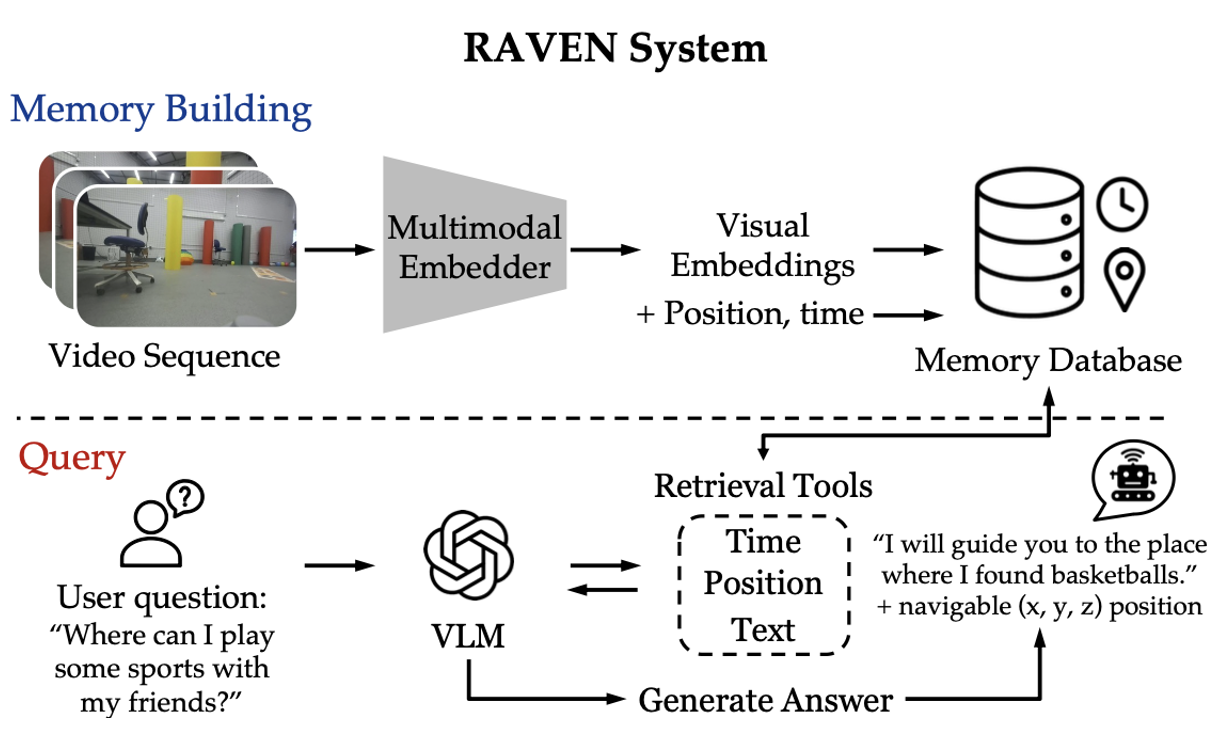
\includegraphics[width=0.85\textwidth]{figures/raven_system.png}
  \caption{The RAVEN system. At ingest time (top), the multimodal
    embedder converts each video frame into a visual embedding stored
    in a vector database alongside the robot's pose and timestamp.
    At query time (bottom), a vision--language model iteratively
    invokes three retrieval tools (text, time, position) over the
    memory database, accumulates evidence, and emits an answer with
    a navigable $(x,y,z)$ position. Reproduced from
    \cite{ref:raven}.}
  \label{fig:raven}
\end{figure}

\subsection{Contributions}

This independent work makes three scoped contributions, each
addressing a specific gap in the RAVEN open-VLM coverage:

\begin{enumerate}
  \item \textbf{Open-VLM extension of RAVEN on DARPA TIAMAT
    simulation data.}  I integrate four locally-served open VLMs
    (Gemma~3 27B, Gemma~4 31B, Qwen2.5-VL 32B, and Qwen3-VL 32B) into
    the RAVEN harness via Ollama, add per-model YAML configurations
    to the framework, and run each against a Habitat smoke trajectory
    drawn from the DARPA TIAMAT competition stack.

  \item \textbf{A difficulty-stratified evaluation suite (L1--L5).} I
    author a nineteen-question suite over the smoke trajectory in
    which each question is tagged with a capability level: direct
    object recall (L1), indirect attribute mapping (L2), spatial
    reasoning (L3), multi-step inference (L4), and
    negation/disambiguation (L5).  Each level is designed to
    \emph{isolate} a specific RAVEN capability: L4\_3 (``where did the
    agent start its exploration?'') is unanswerable by text retrieval
    alone and forces the time-based retriever; L5\_1 (``find a chair
    that is NOT in the kitchen'') forces post-retrieval filtering.
    Ground truth is multi-position, allowing the evaluator to
    distinguish ``right room, wrong pose'' from ``wrong room
    entirely.''

  \item \textbf{Failure-mode diagnosis.} I produce a qualitative
    readout that identifies the dominant agent-side failure
    patterns---most prominently \emph{retrieval loops} in which the
    VLM re-issues the identical query four to six times rather than
    diversifying---and propose three framework-level fixes (query
    diversification, coordinate fallback, tool-use priming) that do
    not require retraining the VLM and do not touch the retrieval
    substrate.
\end{enumerate}

This is a \textbf{replication-and-extension study}, not a novel
method.  The retrieval substrate, the tool-use loop, and the
embedder-only baseline are all from the RAVEN paper.  The contribution
here is open-VLM coverage on new evaluation data, the
difficulty-stratified suite, and the failure-mode taxonomy.

% =============================================================================
\section{Background and Related Work}\label{sec:bg}

\subsection{Memory representations for embodied agents}

The literature on long-horizon memory for embodied agents has
converged on three approaches, each with a known failure mode.

\textbf{Closed-vocabulary semantic maps.}  Classical SLAM produces a
metric map; semantic SLAM tags map elements with discrete object
labels drawn from a fixed taxonomy.  The advantage is compactness and
consistency with downstream planners.  The disadvantage is hard:
out-of-vocabulary objects cannot be retrieved at all, and retraining
the perception stack to add a class is costly.

\textbf{Captioning-based open-vocabulary pipelines.}
ReMEmbR~\cite{ref:remembr} and its descendants embed natural-language
captions of frames rather than the frames themselves.  This solves the
closed-vocabulary problem but introduces the \emph{captioning
bottleneck}: anything the captioner does not say cannot be retrieved.
Fine spatial layout, subtle textures, and unusual object configurations
are systematically lost.  The RAVEN paper's NaVQA experiments show
ReMEmbR underperforms direct visual embedding by 20--30\% on hard
queries.

\textbf{Long-context VLMs.}  Reading every frame at query time
preserves all visual information but does not scale.  Context window
limitations of even the largest VLMs are exceeded at trajectory lengths
of a few hundred to a few thousand frames; cost scales linearly per
query.

\textbf{Recurrent / RNN-based memories.}  Forget over long horizons in
a way that is hard to control or interrogate.

\subsection{The RAVEN system}

RAVEN proposes two design shifts that together address the limitations
above.  First, \textbf{embeddings, not captions}: modern multimodal
encoders (CLIP~\cite{ref:clip}, SigLIP~\cite{ref:siglip},
QQMM-embed-v2~\cite{ref:qqmm}) are sufficiently aligned with language
that raw visual embeddings can be retrieved with text queries,
skipping the lossy image-to-text step.  Second, \textbf{retrieval, not
attention}: instead of passing every stored frame to a long-context
VLM, the agent invokes targeted retrieval over a vector database and
operates on a \emph{working memory} of retrieved frames, achieving
sub-linear retrieval complexity and order-of-magnitude lower per-query
memory pressure.

The RAVEN agent loop maintains a context $R_\tau$ of accumulated
retrieved frames, parses the user query, and at each step either emits
a final answer or issues a retrieval call.  Three retrieval
primitives are exposed:

\begin{itemize}
  \item \textbf{Text-based.}  The VLM proposes a query string
    $\hat{q}$.  The system computes $\hat{z}_q = f_\text{enc}(\hat{q})$
    and returns the top-$K$ frames by cosine distance.  This is the
    workhorse primitive.
  \item \textbf{Time-based.}  Returns $K$ \emph{consecutive} frames
    anchored at a queried timestamp.  The RAVEN paper notes this
    performs better than nearest-neighbor retrieval in time, because
    consecutive frames are more diagnostic of trajectory state.
  \item \textbf{Position-based.}  Returns $K$ spatial nearest
    neighbors to a VLM-proposed coordinate $(\hat{x},\hat{y},\hat{z})$.
\end{itemize}

\begin{figure}[ht]
  \centering
  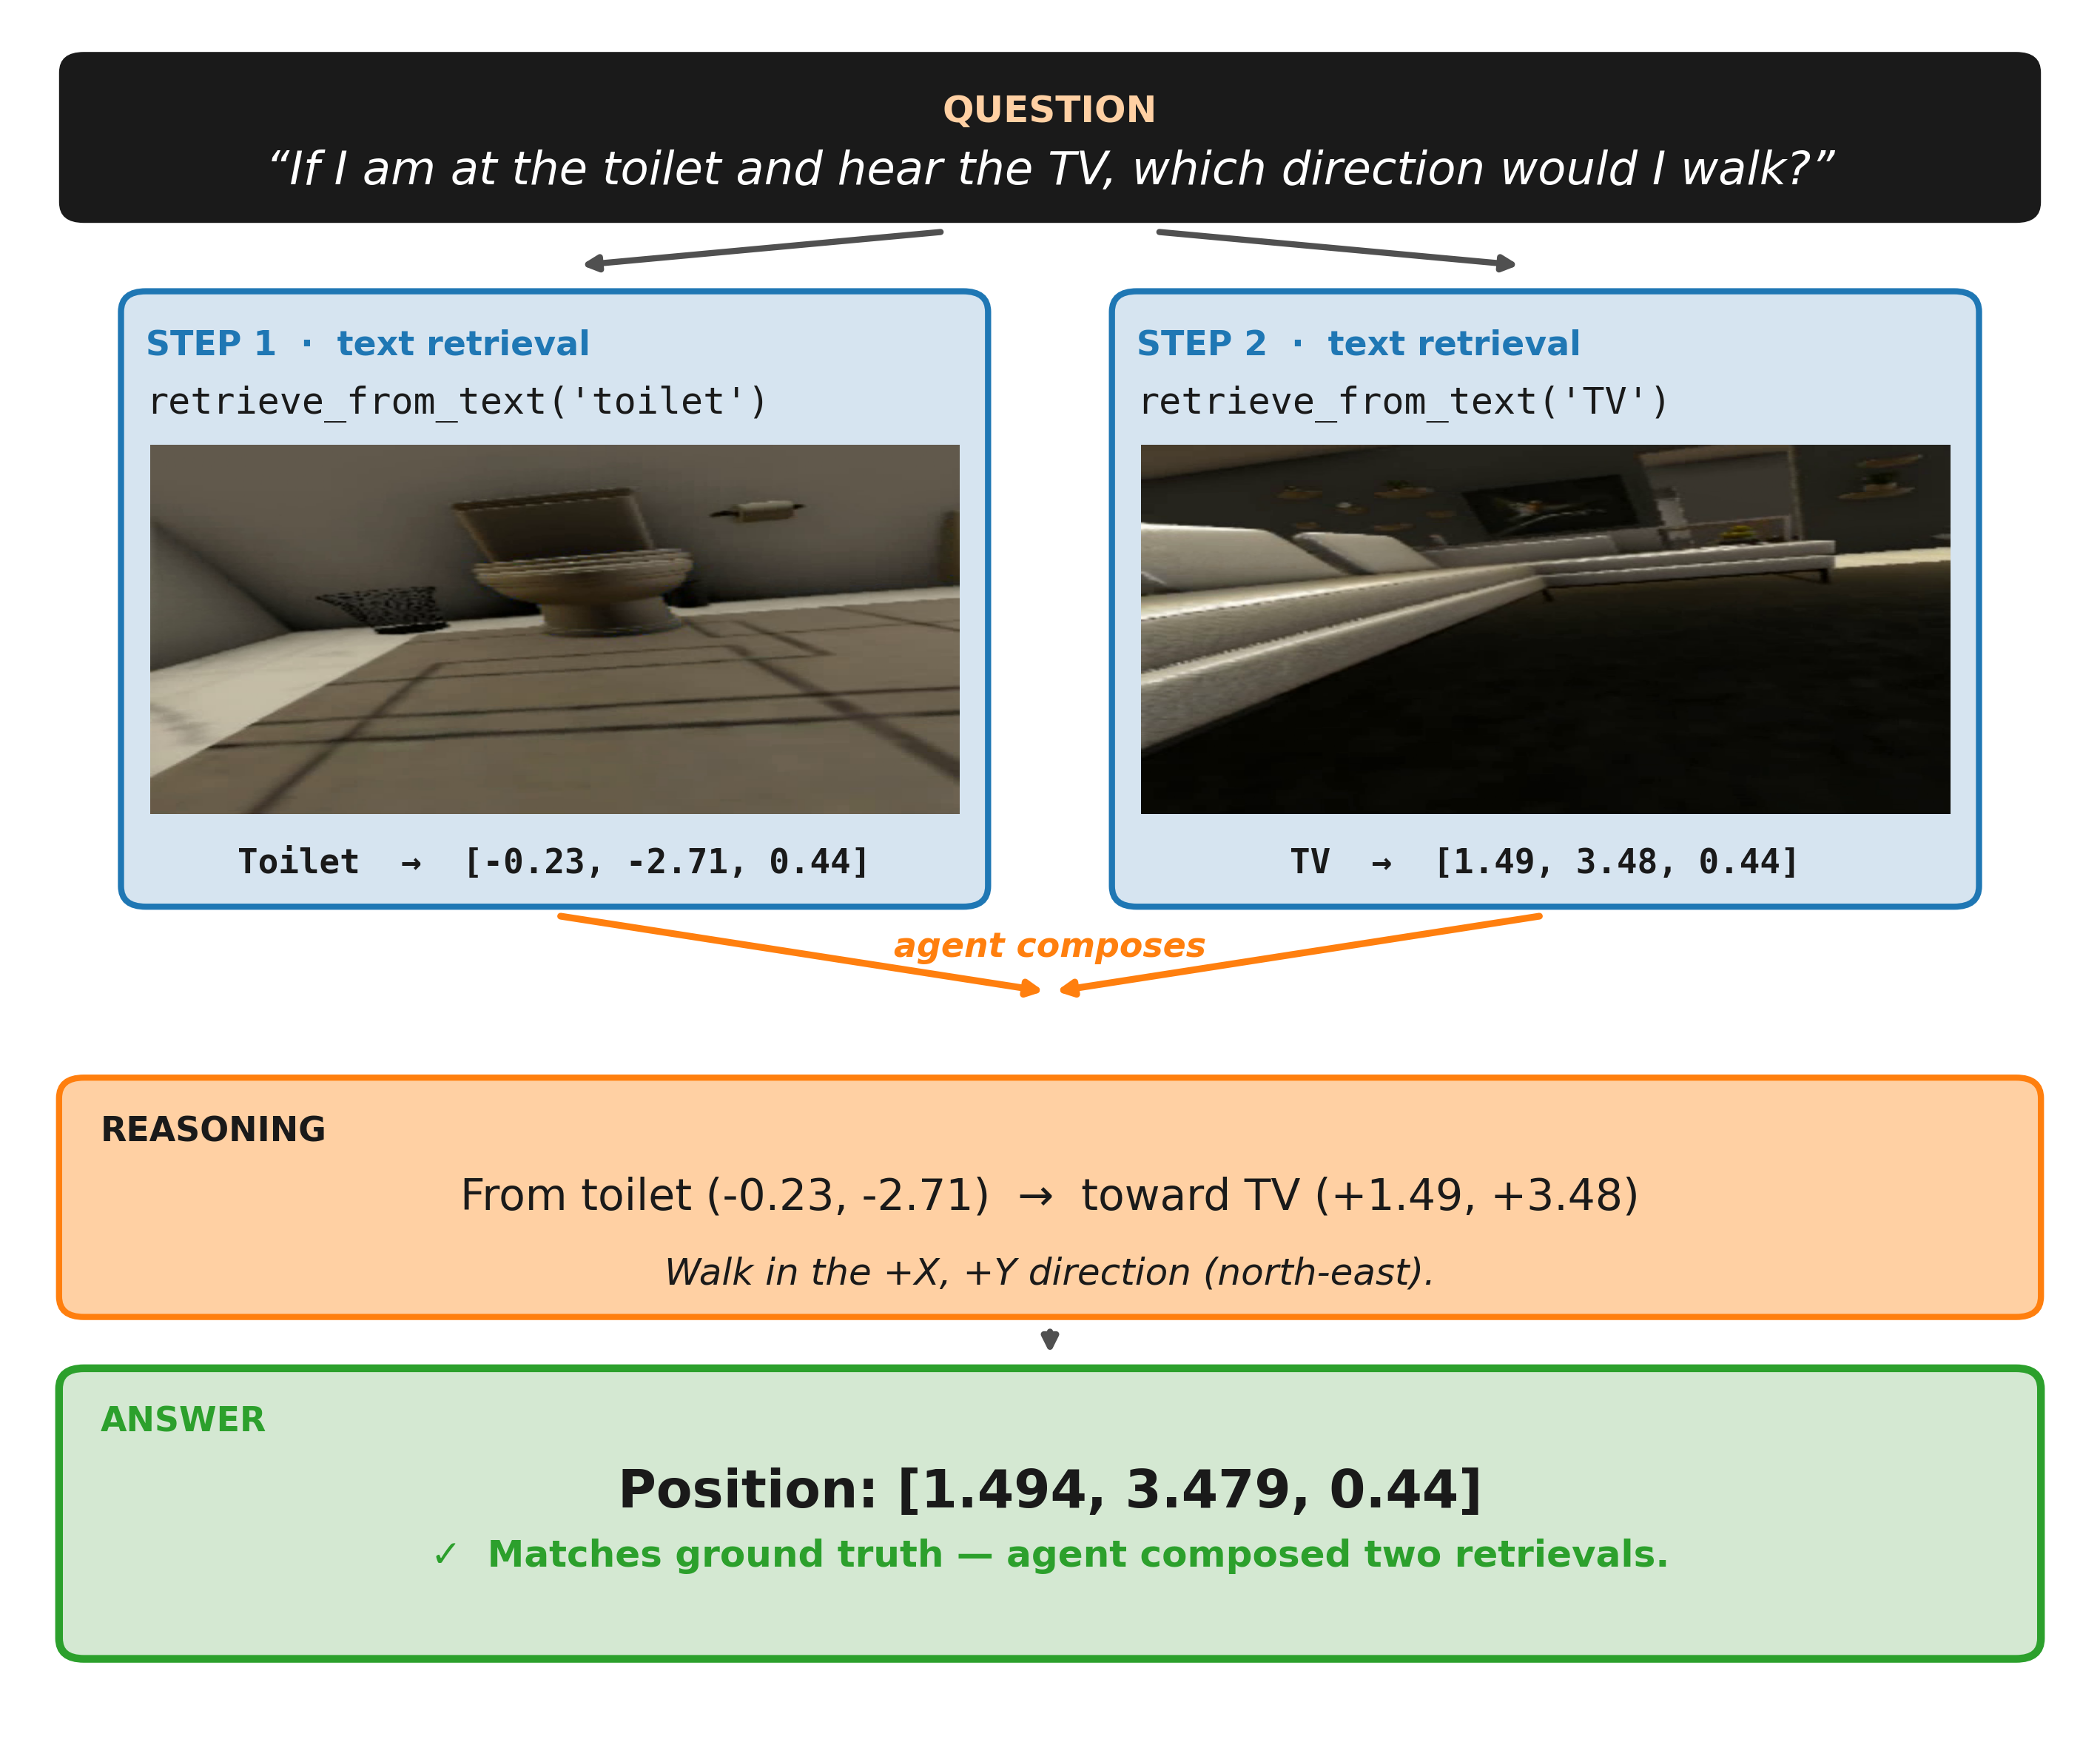
\includegraphics[width=0.85\textwidth]{figures/reasoning_loop.png}
  \caption{RAVEN's tool-use loop.  The VLM parses the query, decides
    whether to emit an answer or call a retrieval primitive,
    accumulates evidence in $R_\tau$, and repeats.  The three retrieval
    primitives are exposed as tools.}
  \label{fig:loop}
\end{figure}

The reported results in the RAVEN paper are strong on the closed-VLM
track.  RAVEN with QQMM-v2 outperforms ReMEmbR by up to 30\% on hard
queries; quality is maintained as memory scales to $\sim$3{,}000
frames on the FindingDory long subset (where a VLM-only baseline
degrades sharply); and $\ge97\%$ success is achieved on real Unitree
Go1 rollouts.  The open-VLM concession in \S5.3, however, is the
relevant data point for offline deployment: medium-sized open VLMs
(Gemma3-27B, Qwen3-VL-32B) can drop below embedder-only retrieval on
Habitat-simulation queries, particularly on tasks requiring
multi-step composition.

\subsection{Where this work fits in the literature}

Three nearby lines of recent work each address adjacent questions but
not the one this thesis pursues:

\begin{itemize}
  \item \textbf{Tool-use evaluations of open VLMs.}  Recent work has
    measured how reliably open VLMs invoke tools in general agentic
    settings.  These benchmarks are not embodied; they do not stress
    the visual retrieval substrate.
  \item \textbf{Retrieval-augmented generation (RAG) for VLMs.}
    Adjacent in mechanism but the retrieved corpus is text/document,
    not visuo-spatial-temporal robot memory.  Failure modes do not
    transfer.
  \item \textbf{Habitat / FindingDory~\cite{ref:findingdory} benchmark
    papers.}  Provide standardized question suites over indoor scenes,
    but the published RAVEN evaluation does not break out per-difficulty
    performance for open VLMs at the granularity needed to localize
    failure.
\end{itemize}

This work sits in the gap precisely identified by the RAVEN authors in
\S5.3: \emph{if open-VLM RAVEN is already at or below the
embedder-only floor, what is actually driving the loss?}  The L1--L5
evaluation suite is the instrument designed to answer this.

% =============================================================================
\section{Methods}\label{sec:methods}

\subsection{Environment and base system}

I evaluate inside the \textbf{DARPA TIAMAT} competition stack, using
the \texttt{remembr\_static\_eval\_vlm.py} harness and the
\texttt{darpa\_vlm\_prompts} prompt set.  All code is a fork of the
RAVEN authors' reference implementation; \textbf{no retrieval, tool,
or prompt changes are introduced}.  The only modifications to the
framework are (i)~per-model YAML config additions for the four new VLM
backbones, (ii)~the question file specifying the L1--L5 suite, and
(iii)~the evaluator's grading script.  This scope discipline is
intentional: any performance change must be attributable to the
swapped VLM, not to incidental framework drift.

\subsection{Memory construction}

The \textbf{smoke\_v2} trajectory comprises 843 egocentric Habitat
frames captured over approximately 14 minutes of simulated walking
through an indoor residential scene (entry/hallway, living room,
kitchen, bathroom, dining transition area).  Per-frame poses are stored in
\texttt{position\_data\_habitat\_smoke\_v2.csv} as $(x, y, z,
\text{yaw})$ in scene coordinates.

Each frame is embedded with \textbf{QQMM-embed-v2} (3584-dim;
Hugging~Face: \texttt{youzexue/QQMM-embed-v2})~\cite{ref:qqmm} and
indexed into FAISS~\cite{ref:faiss} alongside the position
$p_i$, orientation $\theta_i$, timestamp $t_i$, and the path to the
on-disk PNG, following the RAVEN \texttt{VLMMemoryItem} schema.
The image bytes themselves are not duplicated into the index; the
path is loaded lazily when the agent retrieves the entry. Top-$K$
is fixed at 5 throughout, using cosine distance.  This matches the RAVEN paper's defaults;
varying $K$ is out of scope.

\subsection{Reasoning backbones}

I integrate four open-source VLMs (Gemma~3 27B, Gemma~4 31B,
Qwen2.5-VL 32B, and Qwen3-VL 32B) by adding YAML configurations that
reference Ollama-served model tags. The harness instantiates each as
the reasoning LLM inside the RAVEN tool-use loop.  Hardware is two
NVIDIA L40 GPUs (each 48~GB VRAM): the Ollama VLM is pinned to
GPU~0; the QQMM embedder runs on GPU~1.

The headline result reported throughout this thesis uses
\textbf{Gemma~4 31B + QQMM-embed-v2}, which is referred to as the
``RAVEN agent'' configuration.  This is the strongest open
configuration that fit fully on the available L40 hardware and is
closest in scale to the medium-open backbones the RAVEN paper concedes
are difficult.

\paragraph{Memory footprint of the open VLM backbones.}
Every backbone in this study is loaded as a 4-bit quantized build;
the unquantized BF16 weights of a 32B-parameter VLM are roughly
64~GB and do not fit on a single L40 at all.  Table~\ref{tab:vlmspec}
reports the approximate VRAM footprint for each backbone, sourced
from published model cards and standard GGUF/Ollama load sizes for
the relevant 4-bit quantization (Q4\_0 or q4\_K\_M).  These are not
\texttt{nvidia-smi} measurements taken in this work; they are
representative numbers from the model providers and community
deployments, and they are reported here only to show that all four
backbones fit comfortably on a 48~GB L40 with substantial KV-cache
headroom.  The footprints cluster in a tight 16--22~GB band despite
the models spanning 27--32B parameters, because 4-bit quantization
compresses weights into roughly the same per-parameter footprint
regardless of family. Gemma~3 27B is the smallest at $\approx$16~GB;
Gemma~4 31B and Qwen3-VL 32B both sit near 20~GB; Qwen2.5-VL 32B is
intermediate at $\approx$19~GB. The footprint differences are small
enough that ``which model fits'' is \emph{not} the operative
constraint, and the performance differences reported below cannot be
charged to memory-headroom artifacts.

\begin{table}[ht]
  \centering
  \caption{Approximate VRAM footprint of the four open VLM backbones
    when served via Ollama in 4-bit quantized form.  Numbers are
    sourced from each model's published card and from
    community-reported load sizes for the relevant quantization;
    they are not measured at runtime in this work.  All four fit
    comfortably on a single 48~GB L40 with substantial KV-cache
    headroom for the tool-use trace.}
  \label{tab:vlmspec}
  \small
  \begin{tabular}{@{}lcc@{}}
    \toprule
    Model (Ollama tag) & Quantization & Approx. VRAM \\
    \midrule
    \texttt{gemma3:27b}                     & q4\_K\_M & $\approx$16~GB \\
    \texttt{gemma4:31b}                     & Q4\_0    & $\approx$20~GB \\
    \texttt{qwen2.5vl:32b-q4\_K\_M}         & q4\_K\_M & $\approx$19~GB \\
    \texttt{qwen3-vl:32b-instruct-q4\_K\_M} & q4\_K\_M & $\approx$20--22~GB \\
    \bottomrule
  \end{tabular}
\end{table}

\subsection{Evaluation suite (L1--L5)}\label{sec:suite}

I author a nineteen-question, five-level suite over the smoke\_v2
scene specifically designed to isolate the pipeline capabilities the
rest of this thesis tries to localize.

\paragraph{Why stratify by capability.}
The thesis is asking \emph{where along the difficulty curve does the
LLM stop being optional?}, and a single aggregate accuracy number
cannot answer that. Two questions that look syntactically similar can
exercise completely different parts of the pipeline: ``Where is the
purple chair?'' is solved by top-1 keyword retrieval; ``Find a chair
that is NOT in the kitchen'' requires the agent to retrieve
\emph{and then filter}. Pooling them obscures exactly the embedder
floor vs.\ agent ceiling divergence that the rest of \S\ref{sec:results}
sets out to chart. I therefore stratify the suite by structural
capability rather than surface form, so per-level scores read as
\emph{which capabilities are present} rather than as a noisy
aggregate.

\paragraph{Design constraints on the level ordering.}
The L1$\to$L5 progression is therefore organized by the structural
capability each level demands of the pipeline, not by perceived
difficulty: L1 demands only keyword retrieval; L2 adds a
concept$\to$object mapping that the embedder can sometimes handle and
the VLM almost always can; L3 demands relational reasoning over
multiple retrieved frames; L4 demands composition, often involving the
time or position retriever rather than text alone; L5 demands
filtering or exclusion over a retrieval set, which neither the
embedder nor a single forward pass can produce.  Each level is
constructed so that a system passing L$k$ must in principle have all
the capabilities required by L$(k{-}1)$---a monotone-capability
ordering, not a difficulty-rating curve.  This makes the per-level
breakdown in \S\ref{sec:perlevel} interpretable as a \emph{capability
ladder}: the level at which an embedder-only or agent configuration
first stops scoring is a direct readout of the missing capability,
not a noisy aggregate.

\paragraph{Adversarial questions.}
Three of the nineteen questions, all at L4--L5, are
\emph{adversarial} to a single RAVEN component and designed to fail
unless that component is exercised correctly: L4\_3 (``Where did the
agent start?'') cannot be solved by text retrieval and forces the
time retriever; L5\_4 (``Where did the agent spend the most time?'')
forces temporal-statistical reasoning over the trajectory rather than
per-frame retrieval; L5\_1 (``a chair that is NOT in the kitchen'')
forces post-retrieval filtering, which a confident top-1 retrieval
will get wrong. L1--L3 contain no adversarial questions by design,
because those levels are meant to measure the joint
embedder+VLM ceiling on lookup-style queries rather than to stress
specific framework components.  The three adversarial cases are what
let the failure-mode diagnosis in \S\ref{sec:failures} attribute
losses to specific framework components rather than to ``the agent
in general.''

\begin{table}[ht]
  \centering
  \caption{The five-level evaluation taxonomy. Each level isolates a
    capability; three questions across L4--L5 are specifically
    adversarial to a single RAVEN component (L4\_3, L5\_1, L5\_4).
    L1--L3 contain no adversarial questions by design.}
  \label{tab:levels}
  \small
  \begin{tabularx}{\textwidth}{@{}llXX@{}}
    \toprule
    Level & Name & Capability probed & Example \\
    \midrule
    L1 & Direct & Object recall from keyword & Where is the purple chair? \\
    L2 & Indirect & Concept $\to$ object mapping & Where can I sit down comfortably? \\
    L3 & Spatial & Relational reasoning over scene & What room is closest to the entry? \\
    L4 & Multi-step & Composed inference (often temporal) & Where did the agent start its exploration? \\
    L5 & Negation & Filter / exclusion over retrieval & Find a chair that is NOT in the kitchen. \\
    \bottomrule
  \end{tabularx}
\end{table}

L1, L3, L4, and L5 contain four questions each; L2 contains three,
for a total of nineteen scoreable questions.  Ground truth is
\textbf{multi-position}: a question may have two or three acceptable
$(x, y, z)$ answers, which lets the grading scheme of
\S\ref{sec:grading} distinguish ``right room, wrong exact coordinate''
from ``wrong room entirely.''
The full text of all nineteen questions, with capability tags and
ground-truth positions, appears in Appendix~\ref{app:questions}.

\subsection{Grading scheme}\label{sec:grading}

Each answer is graded manually against a two-path rubric.  An answer
is \textbf{correct} if \emph{either} path passes:

\begin{enumerate}
  \item Given a predicted position $\hat{p}$ and a ground-truth set
    $\{p^*_j\}$, define $d \;=\; \min_j \|\hat{p} - p^*_j\|_2$.
    The first path passes if $d \le 2\,$m.  The 2-meter threshold
    corresponds to ``same furniture group'' in the test scene.
  \item When the agent returns no coordinate, returns a coordinate
    that fails path~1, or answers a non-positional question (binary,
    text), I manually inspect the retrieved top-$K$ frames and the
    model's response text.  The second path passes if the retrieved
    frames visually show the queried object or room \emph{and} the
    response correctly identifies it.  For non-positional questions,
    this is the only available path: the response text must be
    correct on its merits given the retrieved evidence.
\end{enumerate}

An answer is \textbf{wrong} if both paths fail (i.e., the coordinate
is more than 2~m from any ground-truth pose \emph{and} manual visual
inspection of the retrieved frames does not support the answer, or
the reasoning text is incorrect for non-positional questions).

This rubric is what allows ``right room, wrong pose'' to be graded
distinctly from ``wrong room entirely'' (\S\ref{sec:suite}). A
correct prose answer with no emitted coordinate (e.g., ``the
entryway'') passes the rubric whenever the retrieved frames support
it.  All headline accuracy numbers in this work use this two-path
rubric.

\subsection{Baselines}

Two baselines, both established by the RAVEN paper:

\begin{itemize}
  \item \textbf{Embedder-only.}  Four contrastive image--text encoders
    are evaluated with no LLM in the loop: top-1 retrieval on the user
    query embedding, with the answer coordinate taken as the centroid
    of the retrieved frame's pose.  The four models are CLIP
    ViT-L-14~\cite{ref:clip} (768-dim), CLIP ViT-H-14 (1024-dim),
    SigLIP-384~\cite{ref:siglip} (1152-dim), and
    QQMM-embed-v2~\cite{ref:qqmm} (3584-dim).
  \item \textbf{ReMEmbR}~\cite{ref:remembr}.  Caption-based baseline.
    Quantitative ReMEmbR numbers are inherited from the RAVEN paper's
    reported patterns; this work does not re-run the captioner
    end-to-end on smoke\_v2.
\end{itemize}

% =============================================================================
\section{Experiments and Results}\label{sec:results}

\subsection{Embedder-only baseline}

Mean top-1 retrieval similarity across the nineteen queries for the
four contrastive embedders evaluated:

\begin{center}
  \small
  \begin{tabular}{@{}lcc@{}}
    \toprule
    Model & Dim & Mean similarity \\
    \midrule
    SigLIP-384 (ViT-SO400M-14) & 1152 & 0.108 \\
    CLIP ViT-L-14 (OpenAI) & 768 & 0.205 \\
    CLIP ViT-H-14 (LAION-2B) & 1024 & 0.249 \\
    \textbf{QQMM-embed-v2} & \textbf{3584} & \textbf{0.356} \\
    \bottomrule
  \end{tabular}
\end{center}

\textbf{Observation 4.1.}  QQMM-embed-v2 achieves substantially higher
absolute similarity than CLIP and SigLIP on the DARPA simulation
data---consistent with its navigation-specialized training
distribution.  Among the two general-purpose contrastive embedders,
CLIP achieves approximately twice SigLIP's absolute similarity,
\emph{inverting} the relative ordering reported on some web
benchmarks.  This is consistent with a sim-to-real gap: SigLIP's
training distribution is heavier on natural photographs, while
contrastive CLIP generalizes more evenly to the rendered Habitat
imagery.  Within the CLIP-style contrastive family, similarity rises
monotonically with embedding dimensionality (ViT-L-14 at 768-dim
$\to$ ViT-H-14 at 1024-dim $\to$ QQMM-embed-v2 at 3584-dim;
$0.205 \to 0.249 \to 0.356$); SigLIP breaks this trend, suggesting
the dimensionality effect is a within-family capacity signal rather
than a general law---training distribution dominates across families.

\textbf{Observation 4.2.}  Absolute similarities span
$\approx$0.11--0.36, with three of the four embedders sitting below
the $\sim$0.3 typical on real-world benchmarks---a quantitative
fingerprint of the sim-to-real distributional shift that any
deployment on Habitat-rendered data must contend with.

\subsection{RAVEN with open VLM backbones}\label{sec:openvlms}

I ran the full RAVEN agent against the 19-question suite with each of
the four open backbones, all on the same QQMM-embed-v2 retriever, and
graded each answer manually at the retrieval level (was the correct
frame in the top-$K$ retrieval, regardless of how the VLM formatted
its final answer?):

\begin{center}
  \small
  \begin{tabular}{@{}lccc@{}}
    \toprule
    Model & Approx. VRAM & Correct & Wrong \\
    \midrule
    \textbf{Gemma~4 31B}    & \textbf{$\approx$20~GB}  & \textbf{15 / 19} & \textbf{4 / 19} \\
    Gemma~3 27B             & $\approx$16~GB           & 13 / 19          & 6 / 19          \\
    Qwen2.5-VL 32B          & $\approx$19~GB           & 13 / 19          & 6 / 19          \\
    Qwen3-VL 32B            & $\approx$20--22~GB       & 12 / 19          & 7 / 19          \\
    \bottomrule
  \end{tabular}
\end{center}

\textbf{Observation 4.3.}  All four backbones land in a tight
16--22~GB VRAM band, so any performance differences cannot be
attributed to memory headroom or which model fits. Gemma~4 31B
retrieves the correct frame on 15 of 19 questions; the other three
open VLMs cluster at 12--13 / 19. Notably, Gemma~3 27B is the
\emph{smallest} of the four at $\approx$16~GB and still scores
13/19, two questions behind the headline run. Memory footprint and
retrieval-level accuracy do not correlate on this suite (see
Figure~\ref{fig:mem-vs-acc}).

\textbf{Observation 4.4.}  The bottleneck is downstream of retrieval,
in answer formulation, and it shows up across \emph{every} backbone I
tried. The failure modes catalogued in \S\ref{sec:failures} recur in
qualitatively similar form across all four VLMs. The per-level
breakdown in Figure~\ref{fig:lift} shows all four agents alongside
the embedder baseline; latency, tool-call counts, frame-reuse, and
the walked-through reasoning traces in the remainder of
\S\ref{sec:results} are reported for the headline Gemma~4 31B run
only.

\begin{figure}[ht]
  \centering
  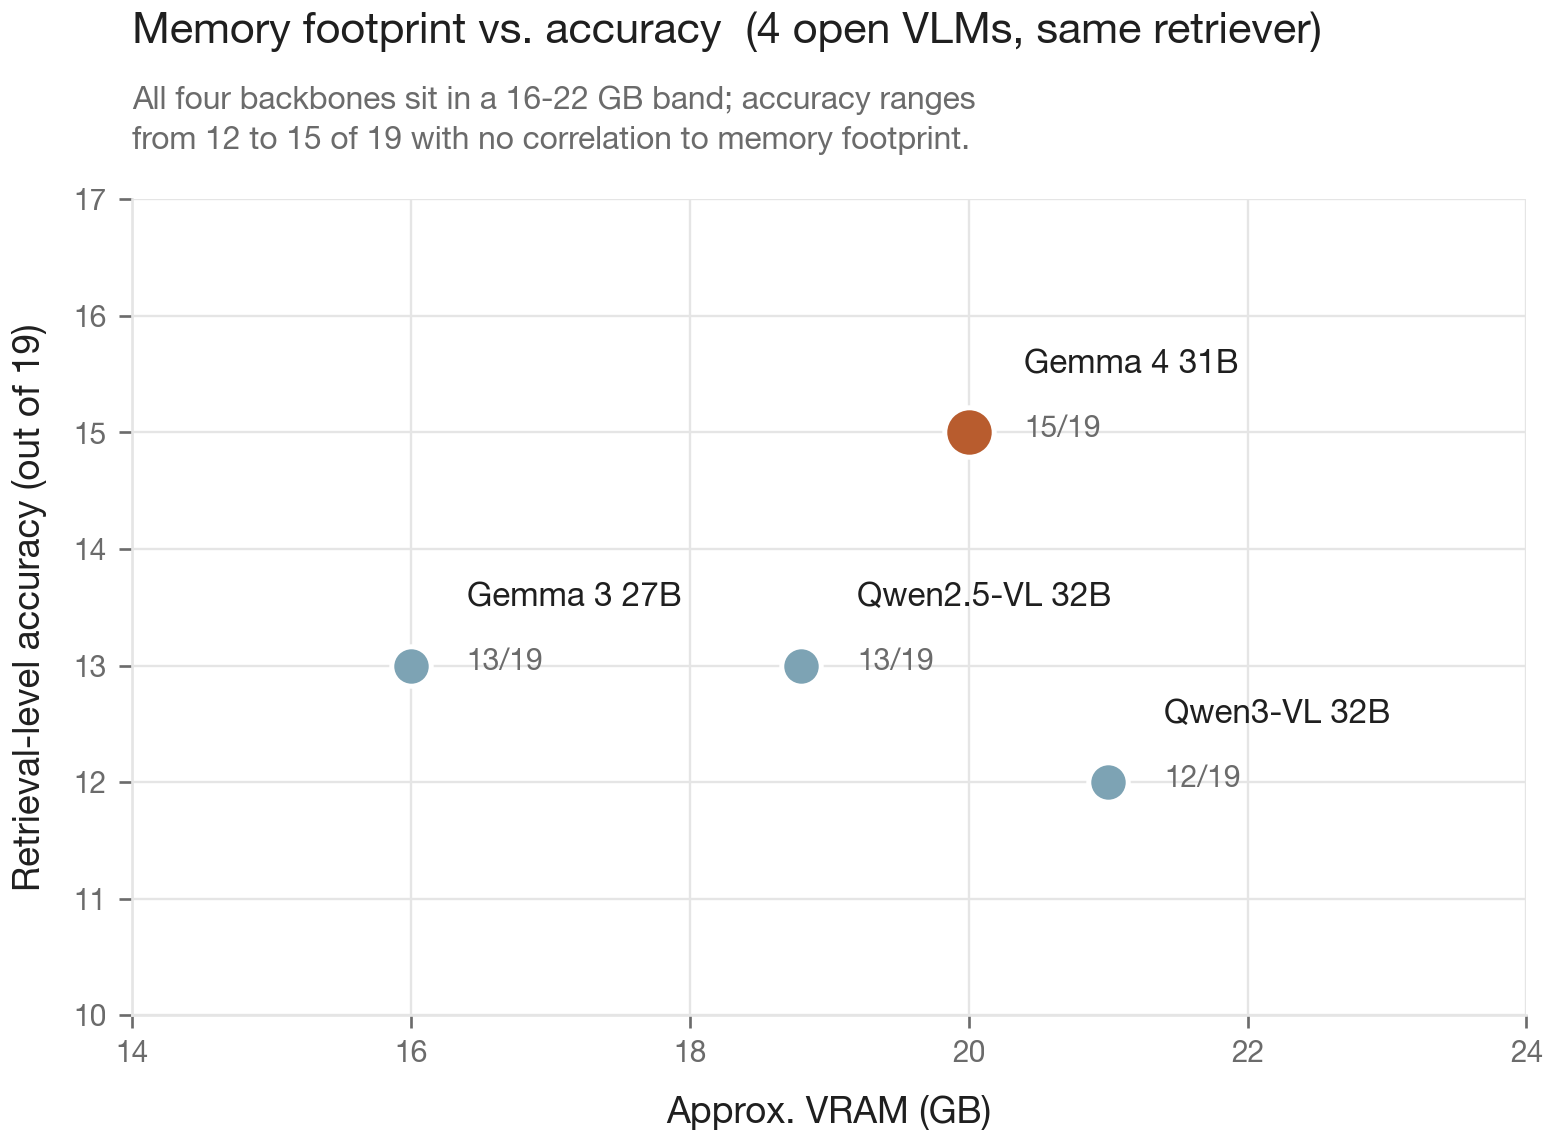
\includegraphics[width=0.65\textwidth]{figures/chart_memory_vs_accuracy.png}
  \caption{Approximate VRAM vs.\ retrieval-level accuracy on the
    19-question suite, for the four open VLM backbones I evaluated.
    VRAM numbers are sourced from published model cards and standard
    GGUF/Ollama load sizes (not measured at runtime in this work).
    All four backbones cluster in a 16--22~GB band and accuracy ranges
    from 12--15 / 19, with no clear correlation: the smallest backbone
    (Gemma~3 27B, $\approx$16~GB) is mid-pack at 13/19, and the
    headline winner (Gemma~4 31B, $\approx$20~GB) is not the smallest.
    Performance differences on this suite cannot be charged to
    memory-headroom or model-fit artifacts.}
  \label{fig:mem-vs-acc}
\end{figure}

\subsection{Per-level breakdown}\label{sec:perlevel}

The single most informative chart in this thesis is the per-level
comparison of QQMM (embedder-only) against each of the four full
RAVEN agents, reproduced in Figure~\ref{fig:lift}.

\begin{figure}[ht]
  \centering
  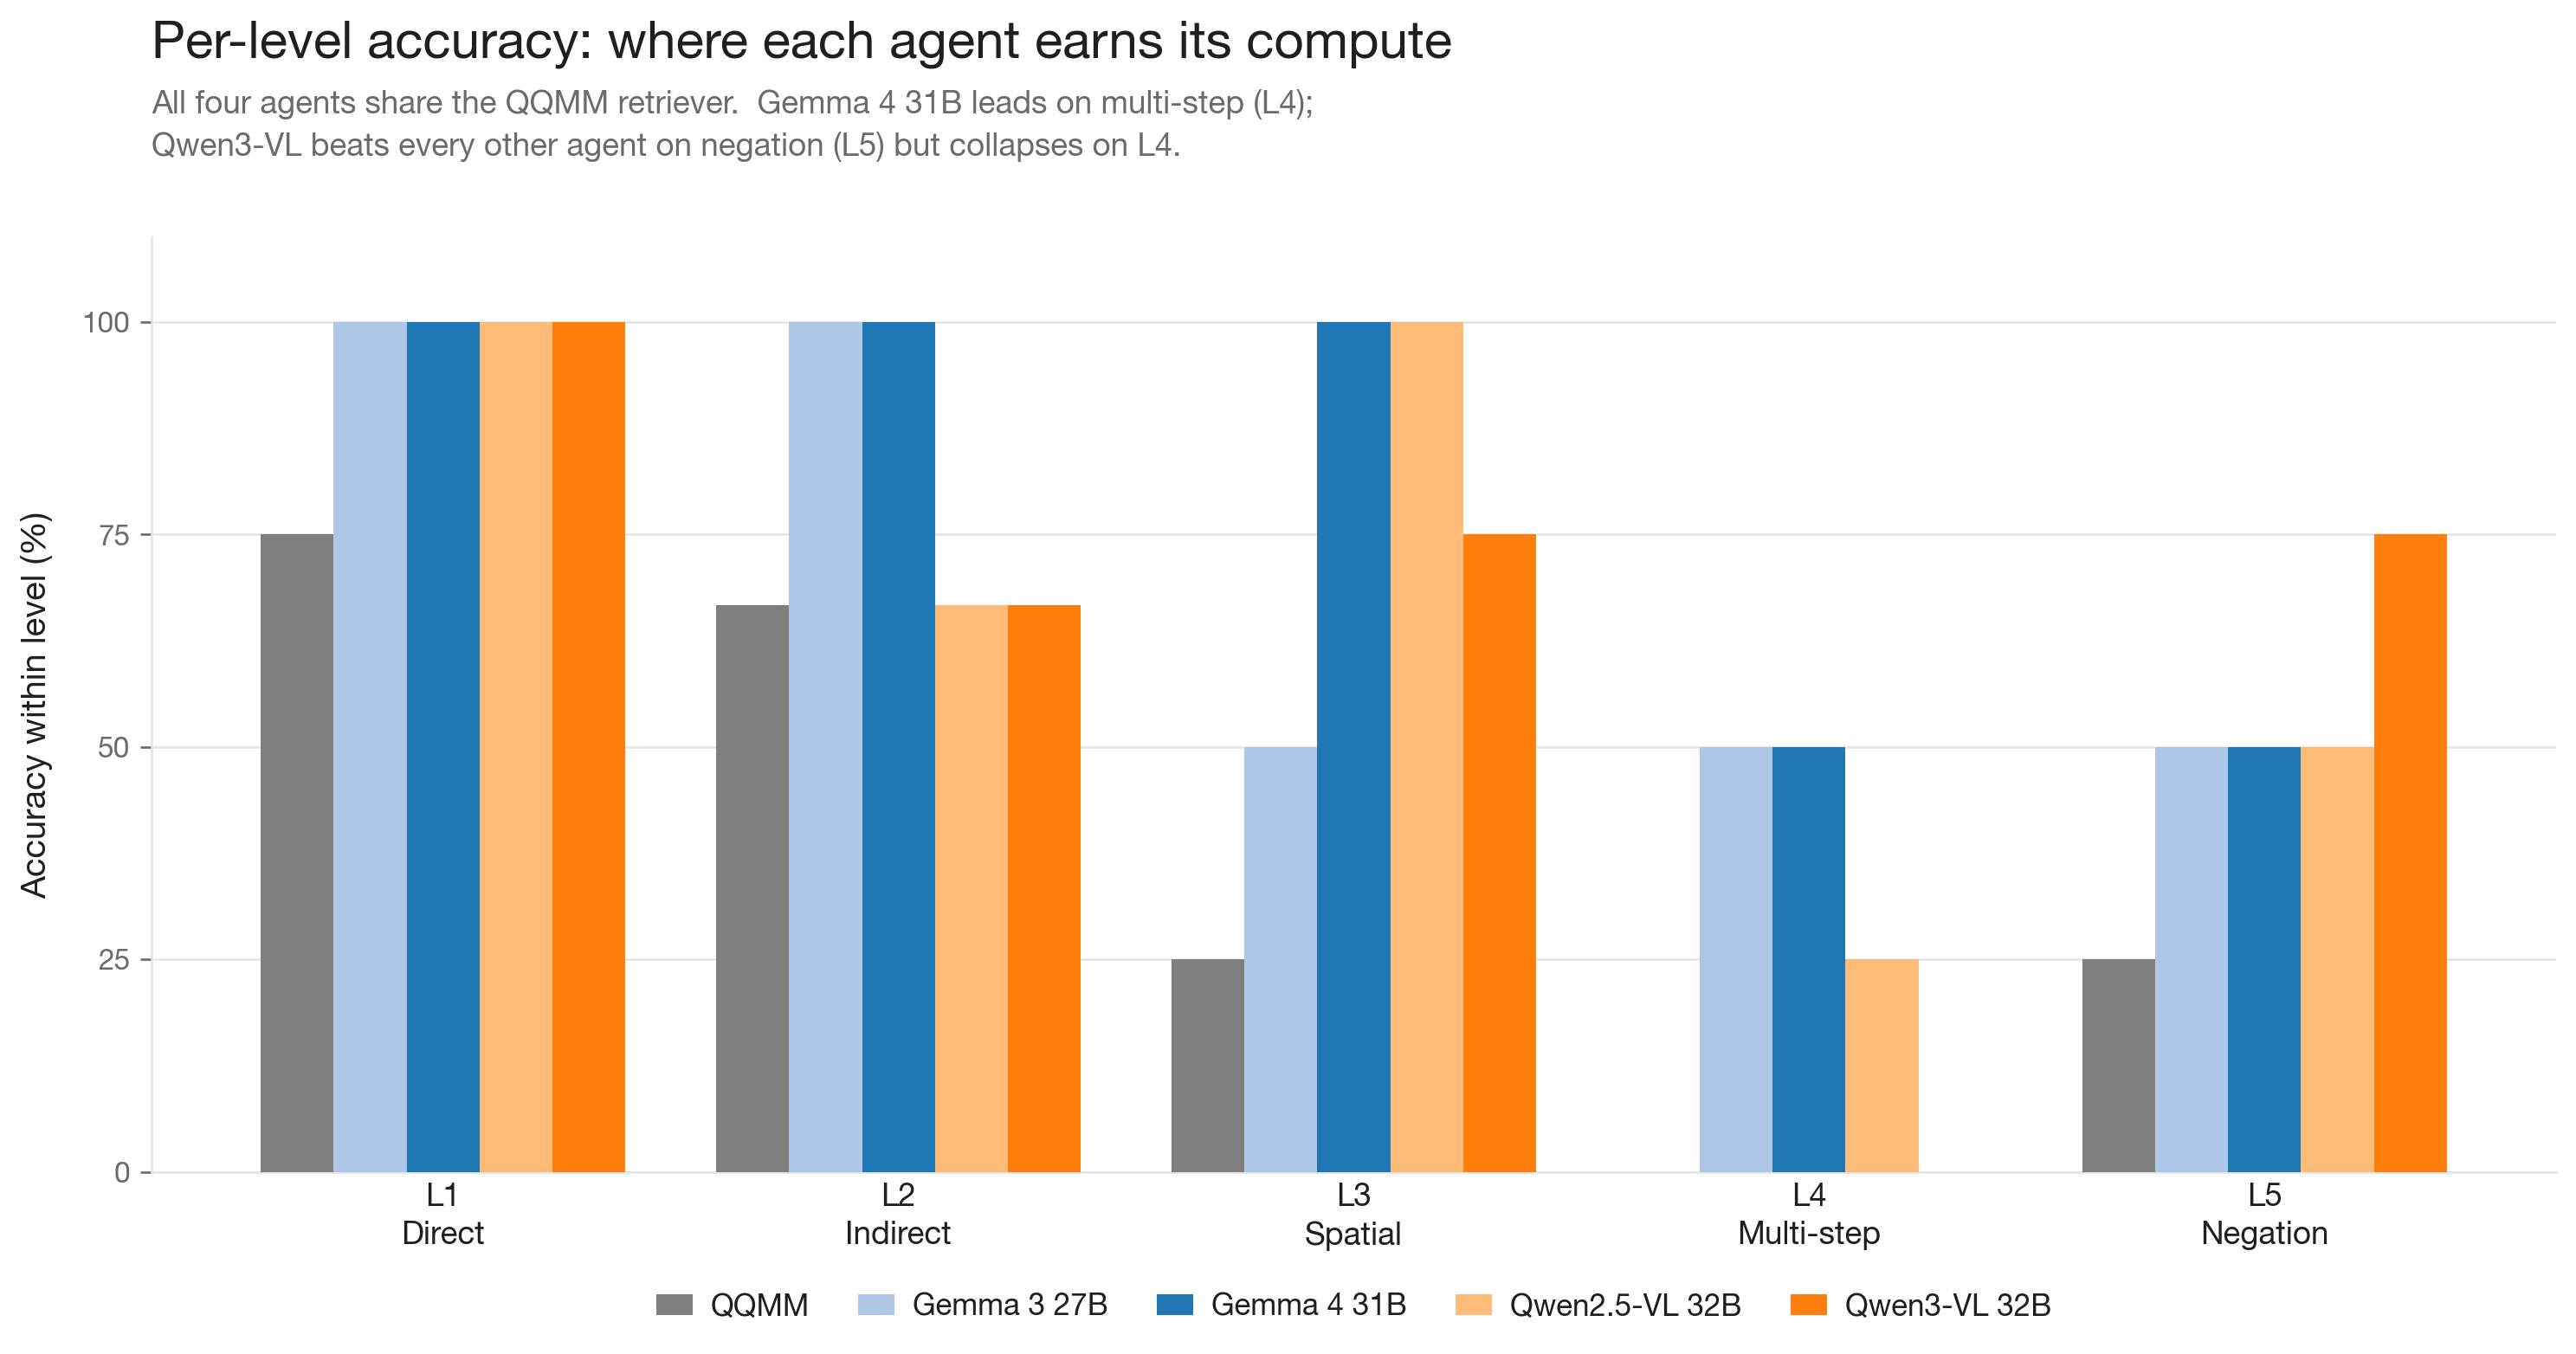
\includegraphics[width=0.95\textwidth]{figures/chart_lift.png}
  \caption{Per-level accuracy across all four RAVEN agents plus the
    QQMM embedder-only baseline.  All four agents share the same
    QQMM retriever, so within-level differences isolate the
    contribution of the VLM.  The agents are tied with the embedder
    at L1 and L2 (the easy half), but each opens a sustained gap on
    L3--L5.  Gemma~4 31B leads on multi-step (L4); Qwen3-VL is the
    only agent above 50\% on negation (L5) but collapses on L4.}
  \label{fig:lift}
\end{figure}

Qualitative agent behavior, level by level (Gemma~4 31B + QQMM):

\begin{description}
  \item[L1 (direct).] Near-ceiling.  All four objects are retrieved in
    top-3 and the model emits coordinates from the retrieved frame's
    metadata cleanly.  The embedder-only pipeline also succeeds on
    L1.  \emph{The VLM adds essentially nothing here}; the scaling
    argument therefore must come from L3--L5.
  \item[L2 (indirect/attribute).] Strong.  The VLM translates ``watch
    the news'' $\to$ \texttt{"television"}, ``sit down comfortably''
    $\to$ \texttt{"comfortable seating"}, ``wash my hands'' $\to$
    \texttt{"sink"}.  Concept-to-object generalization via QQMM
    survives the sim-to-real gap.
  \item[L3 (spatial).] Mixed in raw output, strong in retrieval.  The
    agent produces correct \emph{prose} answers (``the entryway,''
    ``the living room'') in three of four L3 questions, but
    frequently omits coordinates in the answer payload---a framework
    plumbing issue diagnosed in \S\ref{sec:failures}.
  \item[L4 (multi-step).] The standout result is L4\_3---``Where did
    the agent start its exploration?''---the only query in the suite
    where the model spontaneously pivoted off text retrieval.  After
    \texttt{"start of exploration"} returned generic frames, it called
    \texttt{retrieve\_from\_time("00:00:00")} and landed on
    \texttt{frame\_000000}.
  \item[L5 (negation).] The model reformulates rather than filters:
    ``flat surface that is NOT a floor'' $\to$ \texttt{"a flat surface
    like a table or a counter"}.  The agent gets two of four on L5;
    embedder-only gets one of four (a lucky retrieval on L5\_1, where
    top-1 cosine on ``chair'' lands directly on the purple-chair
    frame, which happens to satisfy the negation).
\end{description}

\begin{figure}[ht]
  \centering
  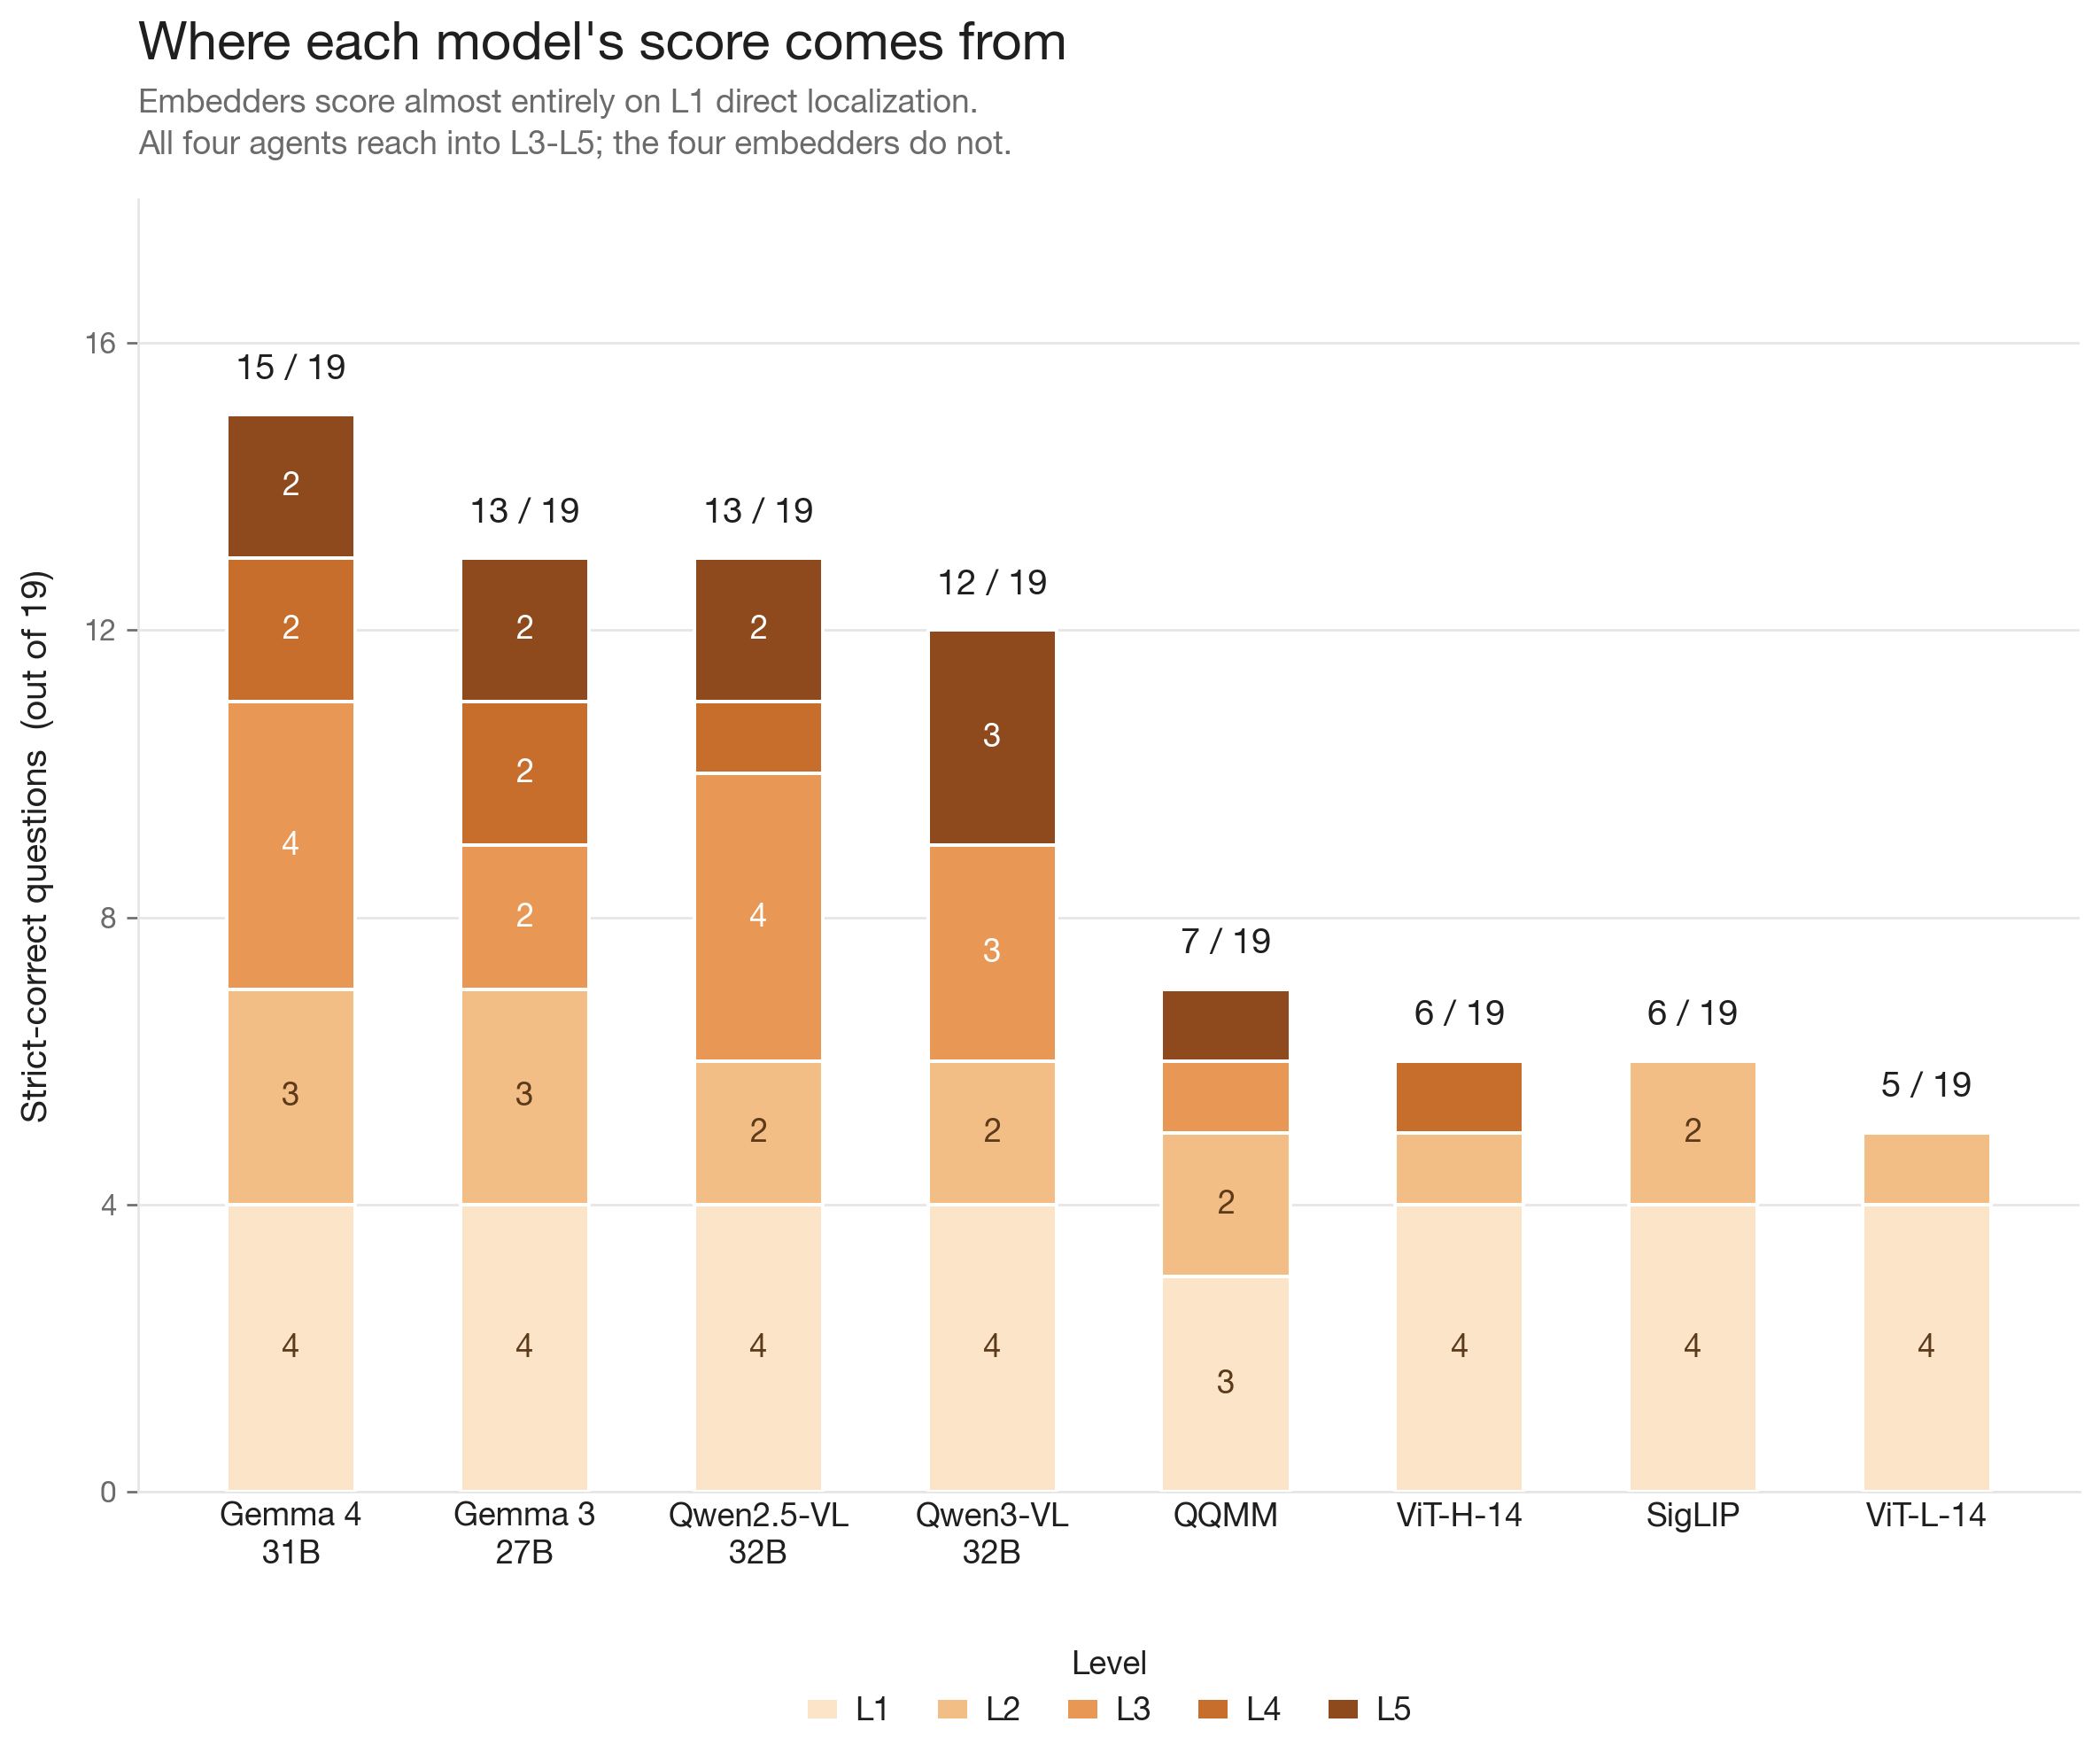
\includegraphics[width=0.70\textwidth]{figures/chart_level_ladder.png}
  \caption{Where each model's score comes from.  One narrow vertical
    column per model (four VLM agents and four embedder baselines),
    segmented by level (L1 light, L5 dark).  Embedders score almost
    entirely on the L1 segment and bottom out from L3 onward; the
    VLM agents are the only configurations that reach L4 with any
    consistency.}
  \label{fig:ladder}
\end{figure}

\subsubsection*{Walked-through reasoning traces}

The per-level summary above is the macro view; the texture of why the
agent succeeds or fails is in the individual traces.  I walk through
three representative cases below.

\paragraph{L4\_2, ``Where would I find something to clean a spill?'' (\checkmark).}
This is the cleanest demonstration of \emph{concept-to-object}
retrieval that the embedder alone cannot do.  The agent issued a
single text retrieval with the query \texttt{"cleaning supplies"} and
the QQMM retriever surfaced \texttt{frame\_000226} (a mop) as the
top-2 result.  The VLM then emitted the mop's pose as the answer.
Embedder-only retrieval on the user's literal query string ``where
would I find something to clean a spill'' lands on irrelevant
kitchen-floor frames; the VLM's reformulation to ``cleaning supplies''
is what makes the retrieval succeed.  This is the L4 win that the
embedder cannot replicate and is consistent with the per-level gap in
Figure~\ref{fig:lift}.

\paragraph{L4\_3, ``Where did the agent start its exploration?'' (\checkmark).}
The standout trace.  The agent first issued \texttt{"start of
exploration"} (a literal paraphrase of the question) and got back
generic indoor frames---no temporal anchor.  Recognizing the failure,
it switched tools: it called
\texttt{retrieve\_from\_time("00:00:00")}, which returns frames
anchored at trajectory start.  The result was \texttt{frame\_000000}
itself, and the agent emitted that frame's pose as the answer.  This
is the only query in the entire suite where a non-text retriever was
spontaneously invoked.  It is positive evidence that open VLMs
\emph{can} orchestrate multi-tool strategies inside RAVEN; the rarity
of this behavior (\S\ref{sec:failures}, item~5.5) is then the
evidence that they don't reach for it without prompting.

\paragraph{L5\_3, ``Find a flat surface that is NOT a floor'' ($\times$).}
The instructive failure.  The agent reformulated the negation rather
than filtering it: it issued
\texttt{"a flat surface like a table or a counter"} as the text query.
QQMM returned \texttt{frame\_000343}, which the VLM correctly
identified as containing marble texture.  However, it then mislabeled
the surface as a ``marble countertop'' when it was in fact a marble
\emph{floor}.  The retrieval was correct in the sense of returning a
visually relevant frame; the \emph{interpretation} of the surface
type was wrong.  This is the texture--surface confusion mode of
\S5.4: the embedder cannot, in general, distinguish horizontal floor
from horizontal countertop because it produces a ``flat marble
surface'' embedding either way.  As \S5.4 argues, the failure
originates at the embedder but a single VLM-level disambiguation
call (``floor or countertop?'') would resolve it without retraining
the retriever.  Reformulation around negation also matters here: an
alternate strategy would have been to retrieve all flat-surface
candidates, \emph{filter out the floors}, and then choose; the
agent did not adopt this strategy.

\paragraph{L4\_4, ``If I'm at the toilet and hear the TV, which direction would I walk?'' ($\times$).}
A different failure mode: retrieval succeeds on the bathroom-side
endpoint but the geometric reasoning step is missing.  The agent
retrieved the toilet (\texttt{frame\_000628}) and described the
living room with the TV in prose, but it never produced a directional
vector or even a unit-bearing answer.
The output was a description of the TV's location, not a direction.
This is consistent with L4\_4 being the hardest L4 question in the
suite: it requires the VLM to do a small geometric computation that
text retrieval alone cannot supply, and the prompt does not prime the
model to do it.

\subsection{Embedding dimension does not crack the ceiling}\label{sec:dim}

A natural hypothesis when an embedder underperforms is ``a bigger
embedder would fix it.'' Figure~\ref{fig:dim} tests this directly
and Table~\ref{tab:dim} reports the underlying counts: across a
4.7$\times$ range of embedding dimensions (768~$\to$~3584),
retrieval-level accuracy creeps up only from 5/19 to 7/19 (26\% to
37\%).  Adding the VLM agent on the \emph{same} 3584-dim QQMM
retriever more than doubles accuracy to 15/19 (79\%) in a single
step.  The retrieval substrate is not the binding constraint.  Note
that the comparison gives the agent two affordances the embedder
baseline does not have---top-$K$ ($K{=}5$) and within-loop query
reformulation---so the +8-question lift bounds the agent's marginal
contribution from above and is partly attributable to those
affordances rather than to the VLM's reasoning alone (\S\ref{sec:limitations}).

\begin{table}[ht]
  \centering
  \caption{Retrieval-level accuracy ($\le 2$\,m or visual-path pass)
    by retriever embedding dimension.  All embedder-only rows use
    top-1 retrieval with no LLM in the loop; the final row swaps in
    the full RAVEN agent (top-$K{=}5$ plus reformulation) on top of
    the same QQMM retriever.  The 4.7$\times$ dimension sweep moves
    only two questions; adding the agent moves eight.}
  \label{tab:dim}
  \small
  \begin{tabular}{@{}lcc@{}}
    \toprule
    Configuration & Embedding dim & Correct \\
    \midrule
    CLIP ViT-L-14 (OpenAI)            & 768  & 5 / 19 \;(26\%) \\
    CLIP ViT-H-14 (LAION-2B)          & 1024 & 6 / 19 \;(32\%) \\
    SigLIP-384 (ViT-SO400M-14)        & 1152 & 6 / 19 \;(32\%) \\
    QQMM-embed-v2                     & 3584 & 7 / 19 \;(37\%) \\
    \midrule
    \textbf{Gemma~4 31B + QQMM (agent)} & \textbf{3584} & \textbf{15 / 19 \;(79\%)} \\
    \bottomrule
  \end{tabular}
\end{table}

\begin{figure}[ht]
  \centering
  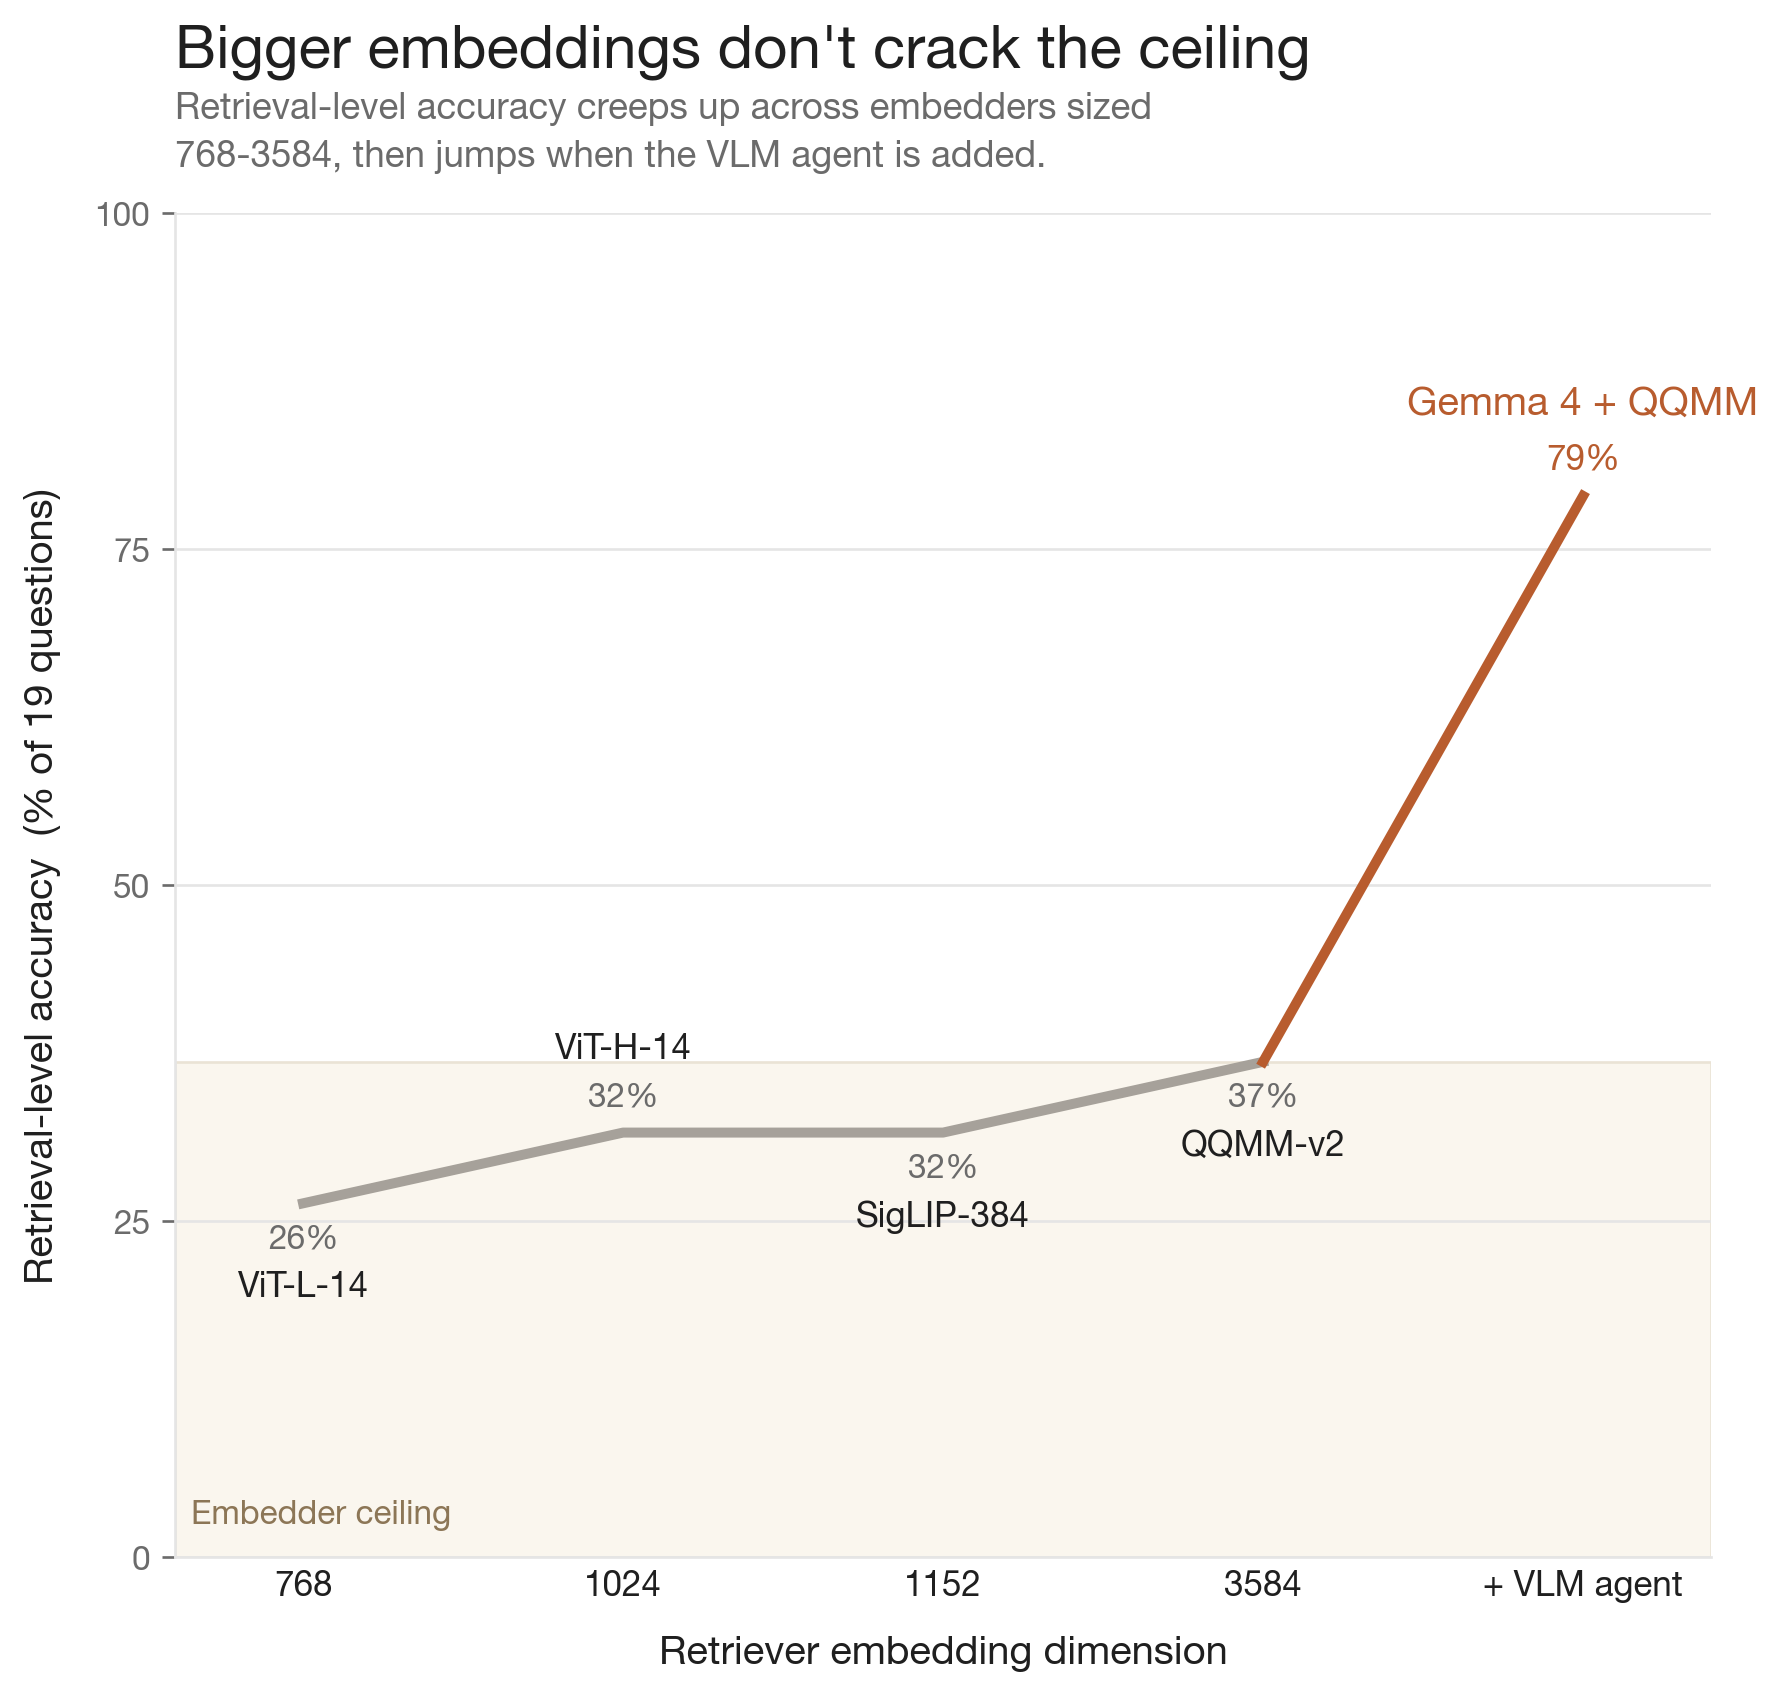
\includegraphics[width=0.65\textwidth]{figures/chart_dim_vs_acc.png}
  \caption{Retrieval-level accuracy as a function of retriever
    embedding dimension.  The four embedder-only configurations
    (left of the dashed step) creep from 26\% to 37\% across a
    4.7$\times$ dimension sweep; adding the Gemma~4 31B agent on top
    of the same QQMM retriever (rightmost point) jumps to 79\%.
    The retrieval substrate is not the binding constraint.}
  \label{fig:dim}
\end{figure}

\subsection{Frame-reuse analysis}\label{sec:framereuse}

A striking qualitative finding in the Gemma~4 31B traces is that the
model consistently re-retrieves the same landmark frames for
semantically related queries.  Three frames each serve four distinct
questions, accounting for 12 of the 19 queries between them; the
remaining seven questions touch other frames once each.
Table~\ref{tab:hubs} enumerates the mapping.

\begin{table}[ht]
  \centering
  \caption{The three ``hub'' frames the \textbf{Gemma~4 31B + QQMM}
    agent re-uses across the suite.  Each row corresponds to one
    canonical landmark frame in the QQMM index; the right column
    lists the four distinct questions for which the agent's top-$K$
    retrieval surfaced this same frame.  Frame-reuse data shown here
    are derived from the Gemma~4 31B run only; equivalent breakdowns
    for the other three open backbones are not reported.}
  \label{tab:hubs}
  \small
  \begin{tabularx}{\textwidth}{@{}lllX@{}}
    \toprule
    Frame & Landmark & \# Questions & Questions answered via this frame \\
    \midrule
    \texttt{frame\_000238} & red/purple chair  & 4 &
      L1\_1 (purple chair),
      L2\_1 (sit comfortably),
      L5\_1 (chair NOT in kitchen),
      L5\_2 (seating closest to bath) \\
    \texttt{frame\_000628} & toilet            & 4 &
      L1\_2 (toilet),
      L2\_2 (wash hands),
      L3\_2 (kitchen $\to$ bathroom),
      L4\_4 (toilet $\to$ TV direction) \\
    \texttt{frame\_000753} & TV / living room  & 4 &
      L2\_3 (watch the news),
      L3\_3 (most furniture),
      L3\_4 (seating that faces TV),
      L4\_4 (toilet $\to$ TV direction) \\
    \bottomrule
  \end{tabularx}
\end{table}

This is interpretable as the VLM maintaining an implicit
\emph{landmark map} of the scene: once QQMM localizes a canonical
frame for an object concept, the agent re-indexes into it across
queries rather than treating each query from scratch.  Notably, the
chair- and toilet-anchored frames each cover questions spanning four
of the five difficulty levels (L1 through L5), which is direct
evidence that re-use is concept-driven---the same physical landmark
is the right answer-anchor whether the query is a direct lookup, an
indirect attribute, a spatial relation, or a negation---rather than
shallow surface-form matching.  This is consistent with RAVEN's
design intent.

\subsection{Latency and tool-call counts}\label{sec:latency}

Two of the qualitative claims in \S\ref{sec:failures}---\emph{retrieval
loops} and \emph{rare multi-tool strategy}---are quantifiable from the
existing run's \texttt{debug\_logs}.  Parsing the Gemma~4 31B + QQMM
log directly:

\begin{itemize}\setlength\itemsep{0pt}
  \item \textbf{Total wall-clock for the suite:} 30.8~minutes (mean
    97~s per question; median 74~s).
  \item \textbf{Latency rises with level:} L1 mean 67~s, L2 66~s,
    L3 100~s, L4 121~s, L5 127~s.  L5\_4 was the slowest single
    question at 228~s.
  \item \textbf{Total tool calls across 19 questions:} 112 text
    retrievals, 3 time retrievals, 0 position retrievals (115 calls
    in total).
  \item \textbf{All 3 time-retriever calls were on L4\_3} (the
    agent-start question).  The position retriever was never invoked
    across the suite, hard quantitative confirmation of the
    \emph{rare multi-tool strategy} pattern in item~5.5 of
    \S\ref{sec:failures}.
\end{itemize}

\begin{figure}[ht]
  \centering
  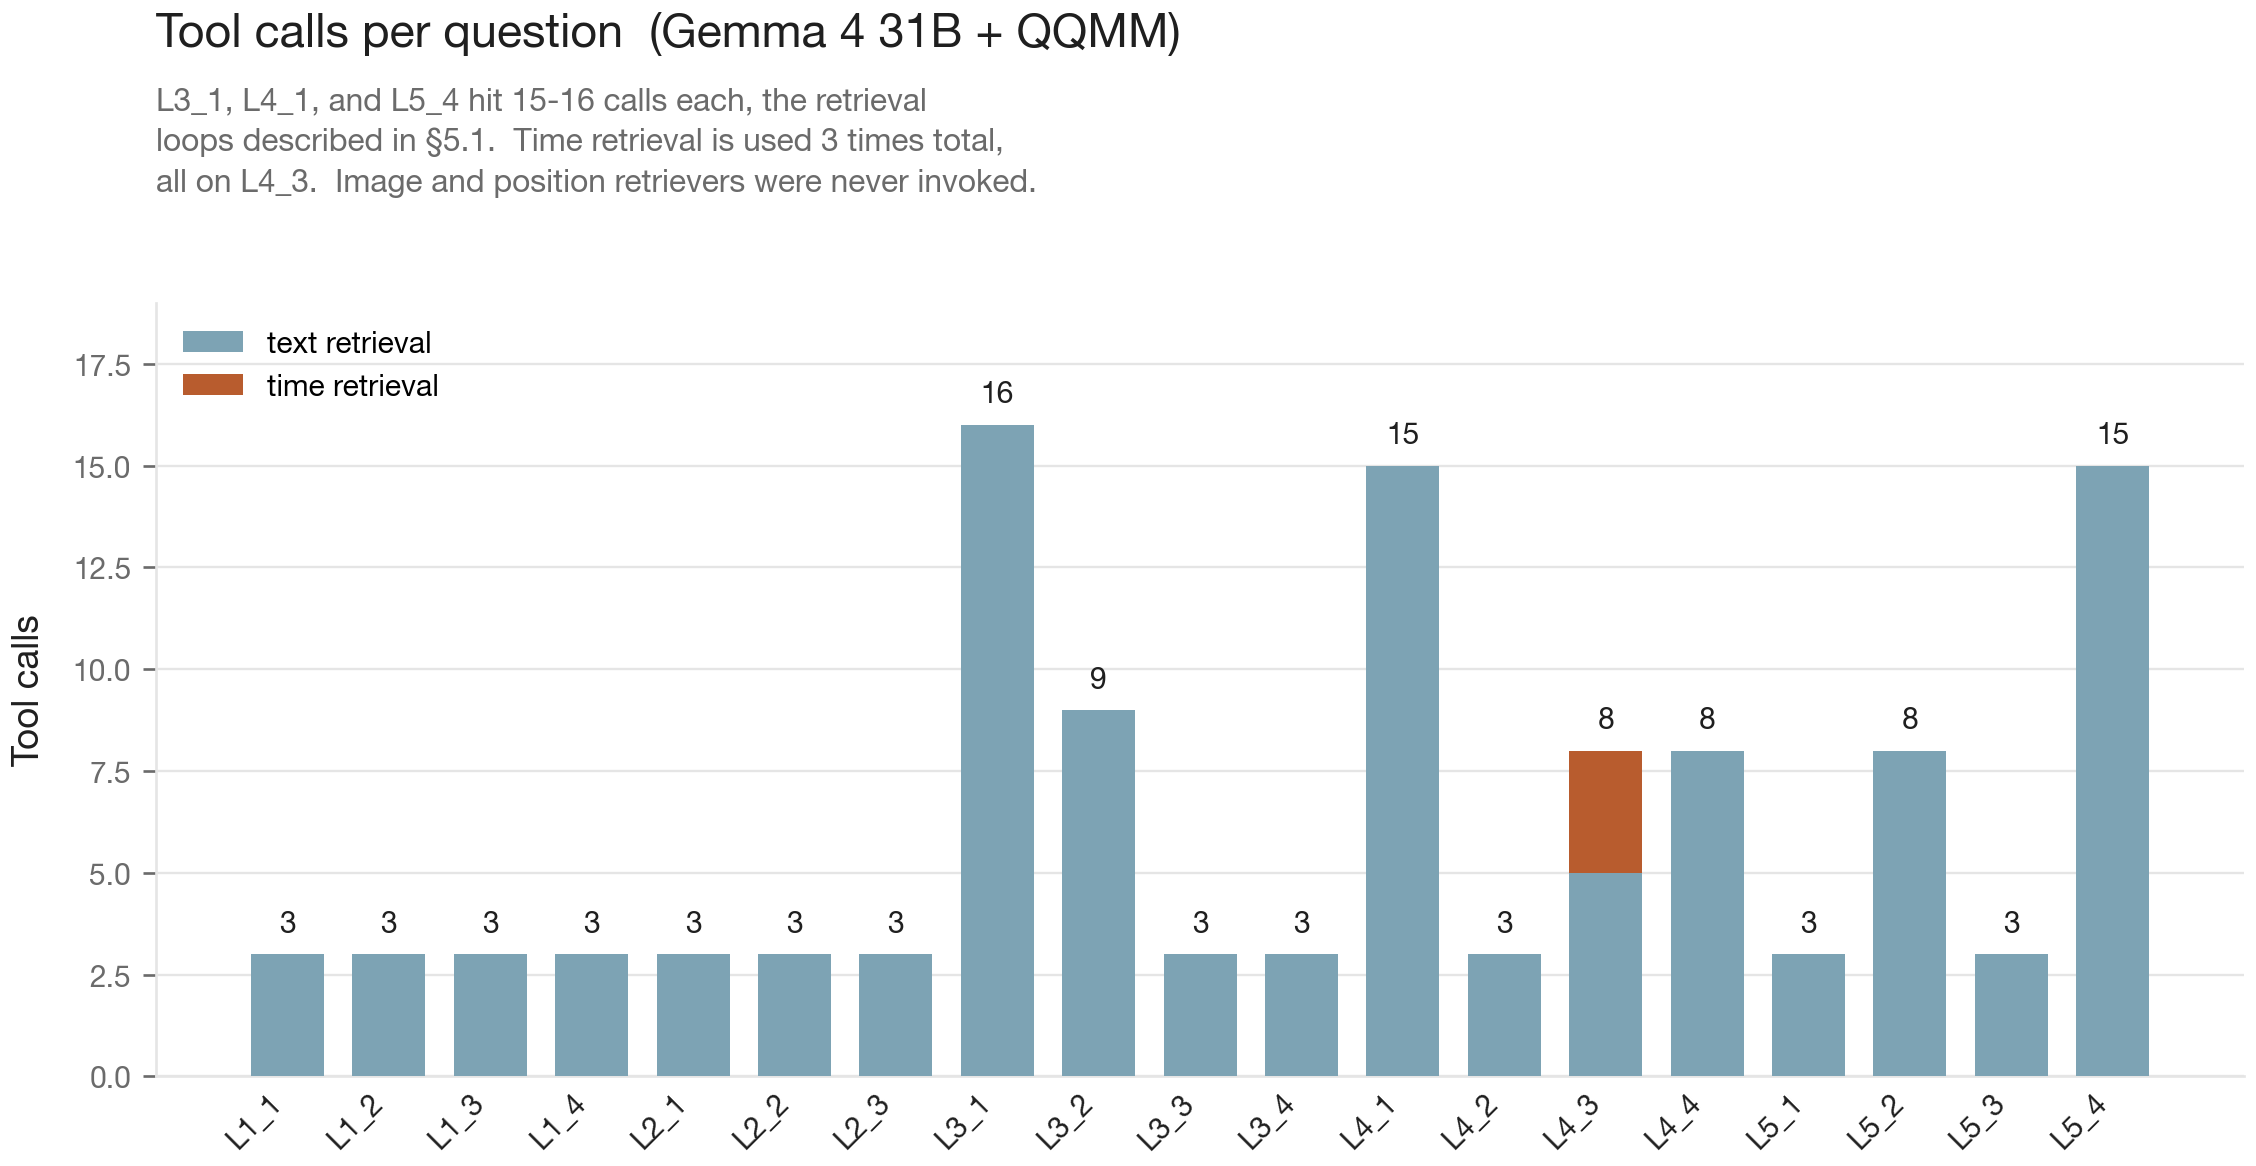
\includegraphics[width=0.92\textwidth]{figures/chart_toolcalls.png}
  \caption{Tool-call count per question (Gemma~4 31B + QQMM).  Most
    questions resolve in 3 calls (one user prompt, one tool
    invocation, one tool response).  L3\_1, L4\_1, and L5\_4 hit
    15--16 calls each---the retrieval-loop pattern of \S5.1, now
    quantified.  Time retrieval is exclusively used on L4\_3.}
  \label{fig:toolcalls}
\end{figure}

\begin{figure}[ht]
  \centering
  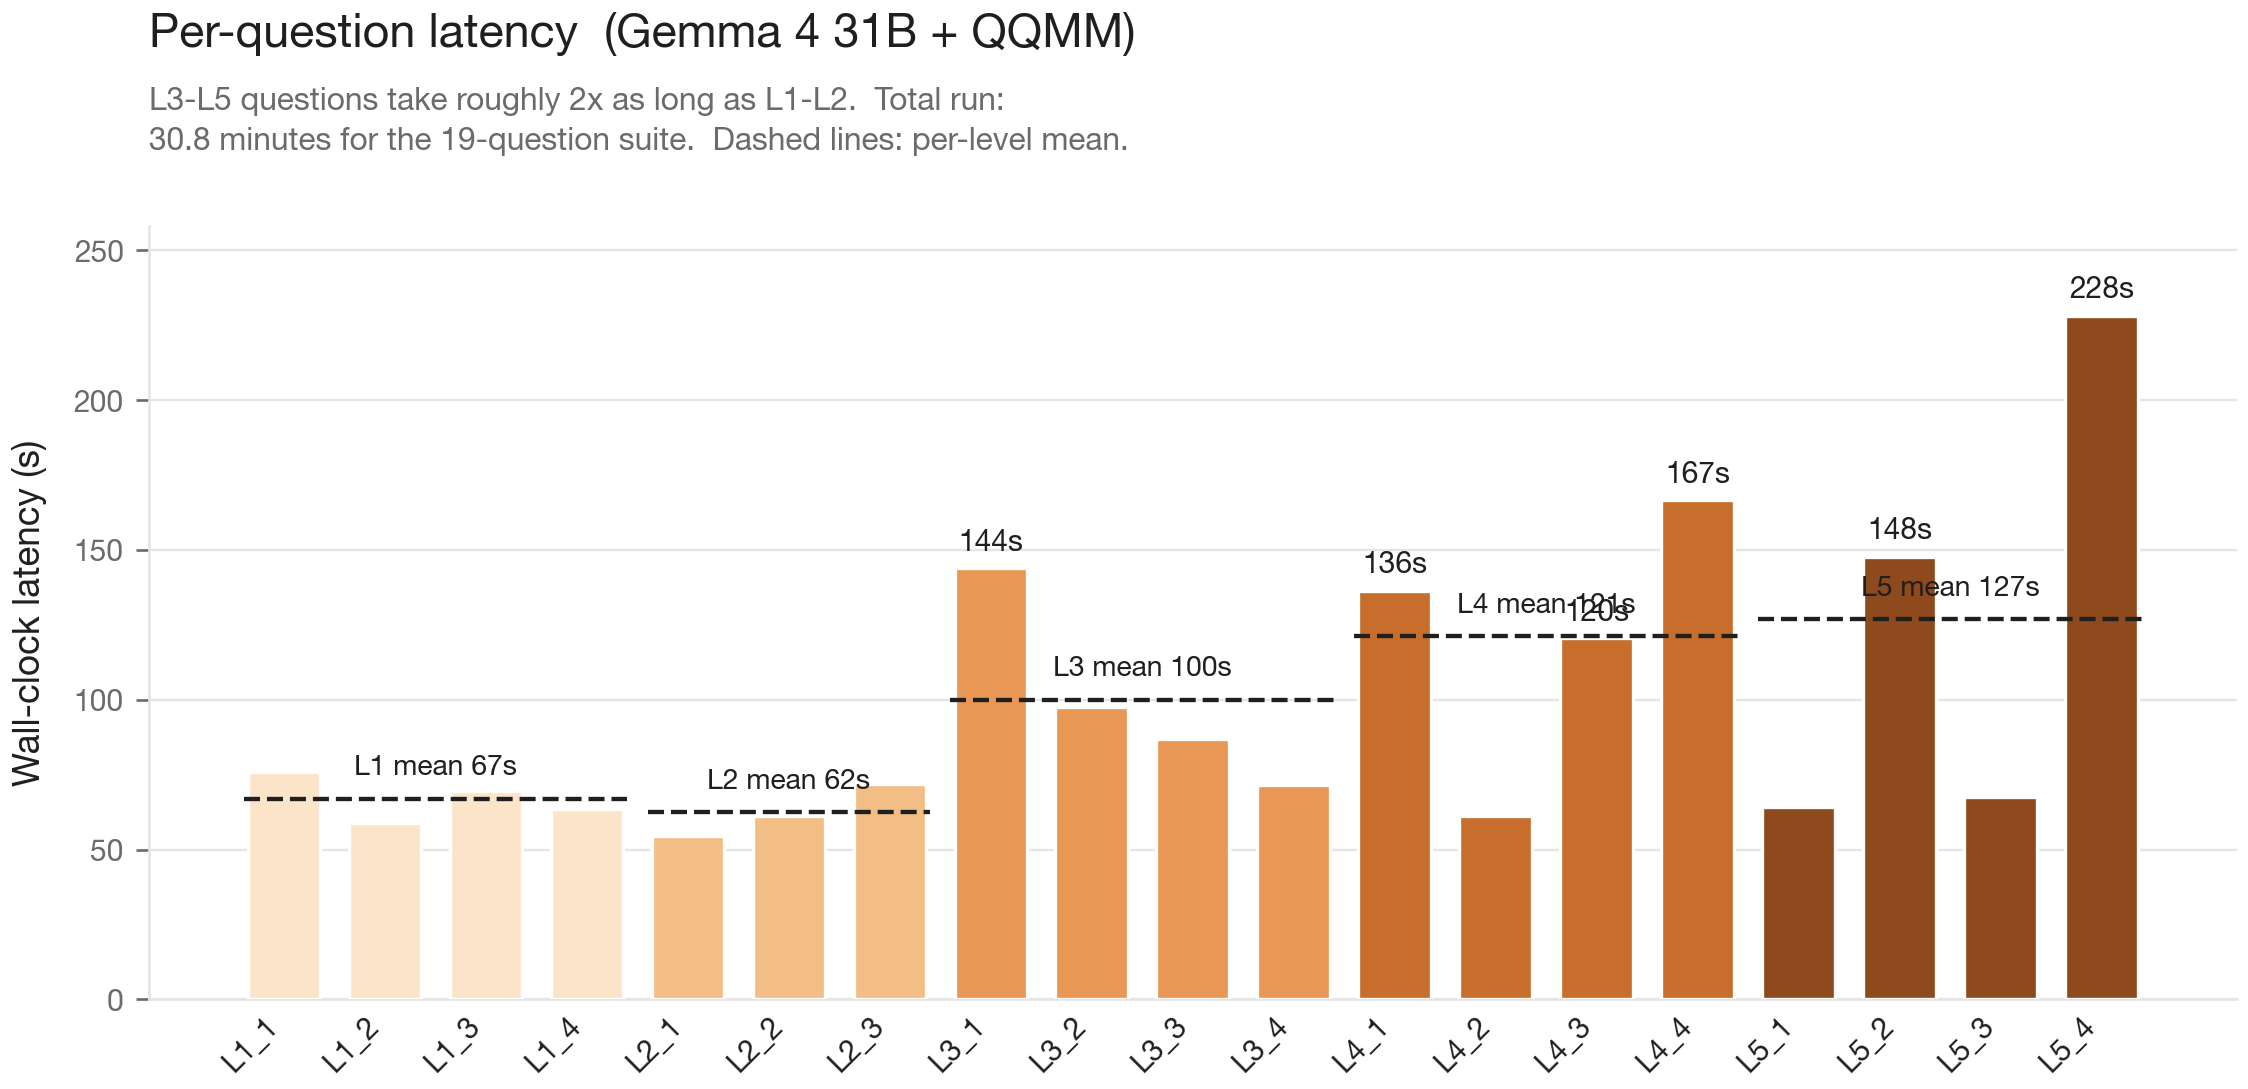
\includegraphics[width=0.92\textwidth]{figures/chart_latency.png}
  \caption{Per-question wall-clock latency (Gemma~4 31B + QQMM).
    L3--L5 questions take roughly twice as long as L1--L2.  The
    distribution is right-tailed: median 74~s, max 228~s.  Dashed
    lines show per-level means.}
  \label{fig:latency}
\end{figure}

The retrieval-loop pattern is now visible as a number rather than an
anecdote: \emph{three} of the nineteen questions account for roughly
two-fifths of the total tool-call budget (46 of 115).  Each of those
three (L3\_1, L4\_1, L5\_4) re-issued the same query 5--6 times before
emitting an answer, and each took $\ge90$~s of wall-clock time.

An L1/L2 question costs about a minute on this hardware; an L4/L5
question costs two.  If a workload is dominated by L1/L2, the
per-query overhead of running the agent at all is the target for
the gating mechanism in \S\ref{sec:future}.

% =============================================================================
\section{Failure-Mode Diagnosis}\label{sec:failures}

The previous section established \emph{that} open-VLM RAVEN tracks
the embedder-only floor on L1--L2 and opens a sustained gap on
L3--L5.  This section asks \emph{why} those L3--L5 results look the
way they do, and where the lever for improvement sits.  I localize
six distinct failure modes; in \S\ref{sec:discussion} I show how
three of them are tractable at the framework layer.

\paragraph{5.1 Retrieval loops dominate the failure cases.}
On the questions that fail, the VLM tends to re-issue the
\emph{identical} query four to six times rather than varying phrasing
or switching retrieval primitives.  I observed
\texttt{"coffee machine"} repeated six times in one L4 trace and
\texttt{"entryway"} repeated six times in another, always returning
the same top-$K$ frames.  The tool-use loop has no backoff, no
query-diversification prior, and no evidence-accumulation criterion
that prevents immediate re-querying.  This is the single most
consequential failure mode.

\paragraph{5.2 Prose-without-coordinates.}
Questions L3\_1 and L3\_3 produced correct \emph{room-level} answers
in prose (``the entryway,'' ``the living room'') but no $(x, y, z)$
coordinate in the answer payload. Under the two-path rubric of
\S\ref{sec:grading} these can still pass via the visual path (the
retrieved frames support the prose answer), but they fail the
coordinate path because no coordinate was ever emitted. This is a
framework failure, not a VLM failure: the VLM ``knew'' the answer;
the answer-formulation path lost the coordinate. A
coordinate-extraction fallback (emit the top-1 retrieved frame's
pose) would salvage every observed case.

\paragraph{5.3 Correct frames, offset coordinates.}
The retrieved frames are right but the reported coordinate drifts
from ground truth by 2--5~meters.  Consistent with a metadata-extraction
bug in the answer-formulation path, not a reasoning failure.

\paragraph{5.4 Texture--surface confusion (embedder-side).}
For L5\_3 (``flat surface that is NOT a floor''), the model correctly
read the marble texture in \texttt{frame\_000343} but mislabeled the
surface as a ``marble countertop'' when it was a marble \emph{floor}.
The retrieval is correct in the sense of returning a visually relevant
frame; the failure is in the \emph{interpretation} of surface
geometry.  Because contrastive image--text encoders are trained against
captions that describe \emph{what is in} a frame rather than
\emph{which surface is which}, two frames containing the same
material---a marble floor and a marble countertop---live in nearly
the same embedding neighborhood.  The encoder cannot, in general,
disambiguate them.

The failure is therefore embedder-side in origin but
\emph{not exclusively embedder-side in remedy}: the agent layer can
in principle close it without changing the retrieval substrate.  A
follow-up VLM call, conditioned on the candidate frame and asking
explicitly ``is the marble surface in this frame a floor or a
countertop?'', would resolve the case in a single bounded inference
because the open VLMs evaluated here \emph{can} read horizontal
versus vertical surface orientation from the image when prompted to
do so.  The structural fix is the same as the cheap-verifier mechanism
proposed in \S\ref{sec:future} for query routing: a verification step
that consults the visual content of the candidate, not just its
embedding similarity, before the answer is emitted.  The embedder
ambiguity is real, but it is not a hard ceiling.

\paragraph{5.5 Rare multi-tool strategy.}
Only 1 of 19 queries triggered a non-text retriever (L4\_3, the
agent-start question; quantified in \S\ref{sec:latency}).  The time
and position retrievers are systematically under-used, implying
that the system prompt or the tool descriptions do not sufficiently
prime the VLM to reach for them when text retrieval fails.  The
fact that the model \emph{can} call them when triggered means the
lever is the prompt, not the model.

\paragraph{5.6 Type-classifier mis-routing (cross-model).}
RAVEN's first reasoning step asks the VLM to classify the question
into one of \{position, text, time, binary\}; a position-typed
answer triggers the coordinate-emission path, while a text-typed
answer skips it entirely. Qwen3-VL on L3\_1 and L3\_3 classified
both questions as \texttt{type=text} (``the question is asking about
which room is closest to the entry, which is a descriptive question
about location''), and then ran a perfectly reasonable text
retrieval that landed on the right frames (\texttt{frame\_000044}
for L3\_1, the living-room frames at \texttt{[8.149,-3.812,0.44]}
for L3\_3) but discarded the position because it had already
committed to a text-only response. This is a different failure
pathway from \S5.2: there, the classifier picks \texttt{position}
and the coordinate is lost downstream; here, the classifier itself
mis-routes the question and the rest of the pipeline correctly
follows from a wrong premise. The lever is the same as \S5.5---the
type-classifier prompt---but the symptom is sharper because no
amount of retrieval-loop tuning can recover a coordinate the agent
decided not to emit.

% =============================================================================
\section{Discussion}\label{sec:discussion}

\subsection{Why the embedder-only floor is high on L1--L2}

The RAVEN paper's negative result---medium open VLMs $\approx$
embedder-only---reproduces on the DARPA simulation data for L1 direct
queries.  The mechanism is now visible: QQMM's top-1 retrieval for a
keyword query already lands on the correct frame, so a VLM that simply
parrots the retrieved frame's location is no better than
retrieval-only.  \textbf{The LLM adds value precisely at L3--L5},
where retrieval alone is insufficient: spatial relationships between
rooms, multi-step composition involving time, and explicit negation.
This is exactly the per-level pattern visible in
Figure~\ref{fig:lift}.  This has a direct deployment implication: if
the workload is dominated by L1-style direct lookups, the LLM is
overhead.  If the workload is dominated by L3--L5, it is essential.

\subsection{What scales with VLM size}

Across the four open backbones (Gemma~3 27B, Gemma~4 31B,
Qwen2.5-VL 32B, Qwen3-VL 32B), retrieval-level scores cluster within
a 3-point band: \textbf{12, 13, 13, 15 out of 19}.  There is no
monotonic scaling trend.  Per Table~\ref{tab:vlmspec}, all four
backbones sit in a tight 16--22~GB VRAM range; the smallest of the
four (Gemma~3 27B at $\approx$16~GB) lands at 13/19, while the
highest-scoring backbone (Gemma~4 31B at $\approx$20~GB) is two
questions ahead at 15/19.  Memory footprint and accuracy do not
correlate.

Scaling the VLM up does not buy retrieval-level accuracy on this
suite, and the headline \S\ref{sec:openvlms} result holds: \textbf{the
bottleneck is downstream of retrieval}.  When an agent fails to
produce a usable coordinate, it has typically retrieved the right
frame but emitted prose without a coordinate, or extracted the wrong
pose from the right frame (\S5.2, \S5.3).  A larger VLM is asked to
do its job more often only because retrieval succeeds more often, but
the framework-level coordinate-emission step has nothing to do with
model size.

The lever for offline open-VLM RAVEN is therefore not the VLM. It is
the answer-formulation layer (\S\ref{sec:recs}).

\subsection{Actionable framework recommendations}\label{sec:recs}

Three changes are tractable at the agent/framework layer, none of
which require fine-tuning the VLM and none of which touch the
retrieval substrate:

\begin{itemize}
  \item \textbf{Query diversification.}  After $K$ consecutive
    identical retrievals (say $K = 2$), force a prompt-level rewrite.
    Breaks the retrieval-loop failure mode (\S5.1).
  \item \textbf{Coordinate fallback.}  When the VLM returns a textual
    room name with no coordinate, emit the top-1 retrieved frame's
    pose. Salvages every observed prose-without-coordinates case
    (\S5.2).
  \item \textbf{Tool-use priming.}  Add few-shot exemplars in
    \texttt{agent\_system\_prompt.txt} specifically showing the time
    and position retrievers being used after an initial text
    retrieval fails.  Addresses \S5.5.
\end{itemize}

None of these three fixes is ablated in this work; their measured
lift is left to follow-up.  Coordinate fallback is the cheapest
(approximately a one-line change in the answer-formatter) and is
the obvious next experiment.

\subsection{Limitations}\label{sec:limitations}

\begin{itemize}
  \item \textbf{Single scene, 843 frames.}  The evaluation is on one
    trajectory; the RAVEN paper's scale claims (up to $\sim$3{,}000
    frames on FindingDory long) are not probed here.
  \item \textbf{Embedder vs.\ agent: not a like-for-like comparison.}
    The headline embedder-only baseline uses top-1 retrieval, while
    the agent has access to top-$K$ ($K{=}5$) and can reformulate
    the query within the loop (\S\ref{sec:dim}).  The +8-question
    lift therefore bounds the agent's marginal contribution from
    above; an embedder + single-shot reformulation baseline (not run
    in this work) would isolate the VLM's reasoning contribution
    more cleanly.
  \item \textbf{Variance not fully quantified.}  I report qualitative
    observations across runs but do not report per-model standard
    deviations.  The RAVEN paper reports $\pm3$--$6\%$ for open VLMs;
    similar variance is expected here.
  \item \textbf{Small-$n$ uncertainty.}  With $n=19$ questions
    overall and $n=3$--$4$ per level, single-question swings move
    the headline number by roughly 5~percentage points and a
    per-level percentage by 25~points. Adjacent embedder rows in
    Table~\ref{tab:dim} that differ by one question (CLIP ViT-L
    5/19 vs.\ ViT-H 6/19) or that tie outright (ViT-H 6/19, SigLIP
    6/19) cannot be statistically distinguished at this sample
    size; the L3--L5 lift pattern, however, spans $\geq 8$
    questions across three levels and is robust to single-question
    swings.  Per-level cells should be read as point estimates
    rather than precise rates.
  \item \textbf{Sim-to-real gap.}  All results are on Habitat-rendered
    frames; the real-robot results in the RAVEN paper are not
    replicated here.
  \item \textbf{Replication, not novel method.}  The retrieval
    substrate, the tool-use loop, and the embedder-only baseline are
    established.  Contribution is open-VLM coverage on new evaluation
    data and the failure-mode diagnosis.
\end{itemize}

\subsection{Key takeaways}\label{sec:takeaways}
\begin{itemize}
  \item \textbf{The lift is the agent, not the retriever.}  Across a
    4.7$\times$ range of embedding dimensions (768 to 3584),
    retrieval-level accuracy varies by 11~percentage points; adding
    the VLM agent on the same retriever lifts it 42~percentage points.
  \item \textbf{The lift is concentrated on L3--L5.}  L1 direct lookup
    is solved by retrieval alone; the agent earns its cost on
    spatial, multi-step, and negation queries where retrieval is
    structurally insufficient.
  \item \textbf{The remaining loss is agent-side and tractable.}
    Three framework-level fixes (query diversification, coordinate
    fallback, tool-use priming) target the dominant failure modes
    diagnosed here without touching the retrieval substrate or
    fine-tuning the VLM.
\end{itemize}

% =============================================================================
\section{Future Work}\label{sec:future}

\paragraph{Routing fast queries around the VLM agent.}
The per-level breakdown of \S\ref{sec:perlevel} shows embedder-only
retrieval is competitive on L1 and adequate on L2, while L3--L5 is
where the VLM agent earns its cost.  The natural next step is to
\emph{route} at inference time, but the design choice is non-obvious.
Retrieval similarity is not a reliable proxy for answer correctness;
the embedder will confidently retrieve visually similar but
semantically wrong frames whenever rooms share furniture or lighting.
A similarity-margin gate alone will short-circuit to wrong answers in
exactly the cases it should defer.  Three candidate gate mechanisms:

\begin{itemize}
  \item \emph{Cheap VLM verifier (draft + verify).}  Embedder retrieves
    a top-1 candidate; a single bounded VLM call decides whether it
    answers the question.  Accepted candidates return immediately;
    rejected ones escalate to the full agent loop.  Costs one cheap
    inference per easy query versus the four-to-six calls of the full
    loop, and the verifier \emph{sees} the candidate so
    confidently-wrong retrievals are caught.
  \item \emph{Multi-signal triangulation.}  Combine retrieval margin,
    a question-shape heuristic, and an answer-shape parse.  All three
    must agree before the gate accepts.  Preserves a true ``no VLM
    call'' fast path but is vulnerable to a wrong frame from a
    similar-looking room passing all three checks.
  \item \emph{Learned classifier on the L1--L5 taxonomy.}  Stretch
    goal; would require a substantially larger labeled set than
    nineteen questions.
\end{itemize}

The cheap-verifier path is the most defensible because it directly
addresses the failure mode that dooms similarity-only gates.

\begin{figure}[ht]
  \centering
  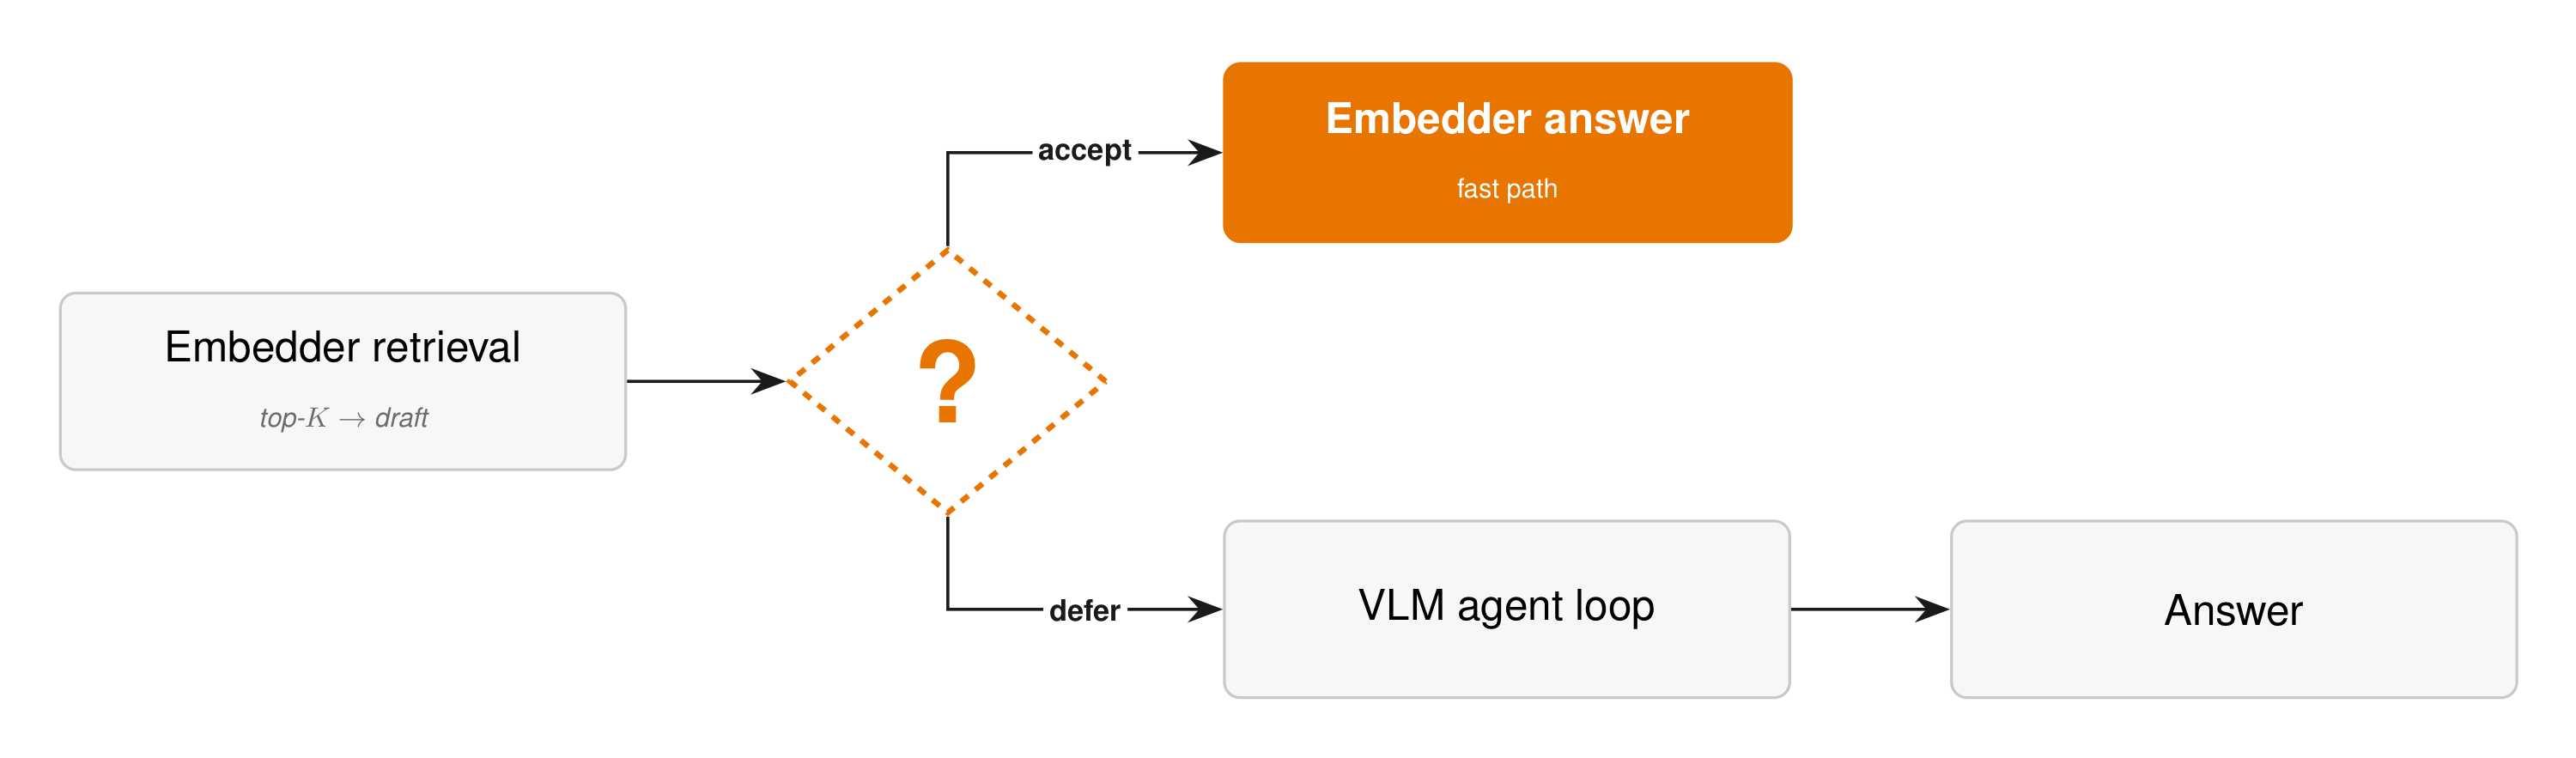
\includegraphics[width=0.85\textwidth]{figures/routing_diagram.png}
  \caption{Proposed routing gate (future work, not in the system
    evaluated in this thesis). The embedder retrieves a top-$K$ draft;
    a gate decides \emph{accept} (return the embedder answer as a fast
    path) or \emph{defer} (escalate into the full VLM agent loop).
    The cheap-verifier mechanism described above instantiates the
    gate with a single bounded VLM call.}
  \label{fig:gate}
\end{figure}

\paragraph{Joint integration with full RAVEN.}
The gate, whichever mechanism, should be added to the full RAVEN
system \emph{jointly} with the \S\ref{sec:recs} recommendations
(query diversification, coordinate fallback, tool-use priming) rather
than as disjoint patches.  The changes interact: coordinate fallback
shortens the agent path the gate is trying to avoid; query
diversification reduces retrieval-loop failures that would cause the
verifier to reject good candidates; tool-use priming changes which
queries are reasoning-required.

\paragraph{Variance and scale.}
Replicate on multiple TIAMAT trajectories and on a FindingDory-sized
memory ($\sim$3{,}000 frames) with per-model standard deviations.

\paragraph{Training-side complement.}
Although the framework-level fixes do not require retraining, a
separate line of work would adapt a smaller open VLM specifically to
the retrieval-loop failure mode: instruction-tuning on synthetic
transcripts that include forced query diversification and
tool-switching.

% =============================================================================
\section{Conclusion}\label{sec:conclusion}

This independent work extended the RAVEN evaluation to locally-served
open-source VLMs over DARPA TIAMAT simulation data, authored a
difficulty-stratified nineteen-question suite specifically designed
to separate retrieval-solvable from reasoning-required queries, and
diagnosed open-VLM failure modes as predominantly \emph{agent-side}
(retrieval loops, coordinate-plumbing gaps, an under-used non-text
retriever, and a question-type classifier that occasionally
mis-routes positional questions into the prose path) rather than
retrieval-substrate or base-VLM failures.

The headline quantitative result is that adding a VLM agent on top of
QQMM-embed-v2 lifts retrieval-level accuracy from 7/19 (embedder-only)
to 15/19 with Gemma~4 31B, with the entire gain concentrated on
L3--L5 (spatial, multi-step, and negation reasoning). Increasing
the embedder dimension by 4.7$\times$ (from 768 to 3584) closes
only 11 percentage points of the gap, while adding the agent closes
42 percentage points. The lift is downstream of the retriever, not
in it.

The practical implication for offline, air-gapped deployments of
RAVEN on open models is direct: most of the gap to closed-VLM
performance is recoverable without retraining, via three
framework-level changes (query diversification, coordinate fallback,
tool-use priming) that target the dominant failure modes identified
here.  The embedder-only pipeline remains a competitive fast path for
L1 queries (consistent with RAVEN's own \S5.3 recommendation), and
the natural next step is to route between fast path and full agent
at inference time using a cheap VLM verifier rather than a
similarity-only gate.

\subsection*{Code and data availability}
All evaluation question files
(\texttt{test\_questions\_smoke.md},
\texttt{test\_questions\_smoke\_qa.json}), per-model YAML configs in
\texttt{cfgs/vlms/}, the modified evaluation harness, and full trace
logs for the headline Gemma~4 31B run are maintained inside the
\textbf{PRISM} project's private GitHub repository, available to
advisers and committee members on request.

% =============================================================================
\begin{thebibliography}{99}
\small

\bibitem{ref:raven}
Y.~Hu, Z.~Zheng, L.~Zha, C.~Xing, R.~Singh, O.~Hossain, A.~Loquercio,
and D.~Shah.
\emph{RAVEN: Long-Horizon Reasoning and Navigation with a
  Visuo-Spatial-Temporal Memory.}
Robotics: Science and Systems (RSS), 2026.

\bibitem{ref:remembr}
A.~Anwar, J.~Welsh, J.~Biswas, S.~Pouya, and Y.~Chang.
\emph{ReMEmbR: Building and Reasoning Over Long-Horizon
  Spatio-Temporal Memory for Robot Navigation.}
IEEE International Conference on Robotics and Automation (ICRA), 2025.

\bibitem{ref:findingdory}
K.~Yadav, S.~K.~Ramakrishnan, J.~Turner, A.~Gokaslan, et al.
\emph{FindingDory: A Benchmark for Memory-Based Navigation.}
2024.

\bibitem{ref:clip}
A.~Radford, J.~W.~Kim, C.~Hallacy, A.~Ramesh, G.~Goh, S.~Agarwal,
G.~Sastry, A.~Askell, P.~Mishkin, J.~Clark, G.~Krueger, and
I.~Sutskever.
\emph{Learning Transferable Visual Models from Natural Language
  Supervision.}
International Conference on Machine Learning (ICML), 2021.

\bibitem{ref:siglip}
X.~Zhai, B.~Mustafa, A.~Kolesnikov, and L.~Beyer.
\emph{Sigmoid Loss for Language-Image Pre-training.}
International Conference on Computer Vision (ICCV), 2023.

\bibitem{ref:qqmm}
Y.~Xue, D.~Li, and G.~Liu.
\emph{QQMM-embed-v2: A Multimodal Memory Embedding Model for
  Visuo-Spatial-Temporal Retrieval.}
Hugging Face: \texttt{youzexue/QQMM-embed-v2}, 2025.

\bibitem{ref:faiss}
J.~Johnson, M.~Douze, and H.~J\'egou.
\emph{Billion-Scale Similarity Search with GPUs.}
IEEE Transactions on Big Data, 2019.

\bibitem{ref:habitat}
M.~Savva, A.~Kadian, O.~Maksymets, et al.
\emph{Habitat: A Platform for Embodied AI Research.}
International Conference on Computer Vision (ICCV), 2019.

\bibitem{ref:gemma}
Gemma Team, Google DeepMind.
\emph{Gemma 3: Open Multimodal Foundation Models.}
Technical Report, 2024.

\bibitem{ref:qwen}
Qwen Team, Alibaba.
\emph{Qwen2.5-VL Technical Report.}
2024.

\bibitem{ref:tiamat}
DARPA TIAMAT Competition documentation.  Internal documentation, 2025.

\end{thebibliography}

% =============================================================================
\appendix

\section{Full Evaluation Question List}\label{app:questions}

The full nineteen-question suite, with capability tags and
ground-truth positions, is maintained in
\texttt{test\_questions\_smoke.md} (human-readable) and
\texttt{test\_questions\_smoke\_qa.json} (machine-readable).  Question
summaries by level:

\paragraph{L1---Direct object recognition.}
\begin{itemize}\setlength\itemsep{0pt}
  \item L1\_1: Where is the purple chair?
  \item L1\_2: Where is the toilet?
  \item L1\_3: Where is the white sofa?
  \item L1\_4: Where are the kitchen cabinets?
\end{itemize}

\paragraph{L2---Indirect / attribute-based.}
\begin{itemize}\setlength\itemsep{0pt}
  \item L2\_1: Where can I sit down comfortably?
  \item L2\_2: Where can I wash my hands?
  \item L2\_3: Where is something I could use to watch the news?
\end{itemize}

\paragraph{L3---Spatial reasoning.}
\begin{itemize}\setlength\itemsep{0pt}
  \item L3\_1: What room is closest to the entry?
  \item L3\_2: Where would I go to get from the kitchen to the
    bathroom?
  \item L3\_3: Which area has the most furniture?
  \item L3\_4: Where is the seating area that faces the TV?
\end{itemize}

\paragraph{L4---Multi-step inference.}
\begin{itemize}\setlength\itemsep{0pt}
  \item L4\_1: I need to make coffee and sit down to drink it.  Where
    should I go first?
  \item L4\_2: If I spill water on the kitchen floor, where would I
    find something to clean it up?
  \item L4\_3: Where did the agent start its exploration?
  \item L4\_4: If I'm at the toilet and hear the TV, which direction
    would I walk?
\end{itemize}

\paragraph{L5---Negation / disambiguation.}
\begin{itemize}\setlength\itemsep{0pt}
  \item L5\_1: Find a chair that is NOT in the kitchen.
  \item L5\_2: There are multiple seating options.  Find the one
    closest to the bathroom.
  \item L5\_3: Find a flat surface that is NOT a floor.
  \item L5\_4: Where did the agent spend the most time during its
    exploration?
\end{itemize}

\section{Per-Model Output Directories}\label{app:outputs}

All runs are reproducible from
\texttt{outputs/smoke\_v2/raven\_results/20q/}:

\begin{itemize}\setlength\itemsep{0pt}
  \item \texttt{gemma4\_31b\_qqmm/}---Gemma~4 31B with QQMM-embed-v2.
    \textbf{Primary result.} Findings summary in
    \texttt{GEMMA4\_31B\_FINDINGS.md}.
  \item \texttt{gemma27b\_qqmm/}---Gemma~3 27B with QQMM-embed-v2.
  \item \texttt{qwen25vl32b\_qqmm/}---Qwen2.5-VL 32B (q4\_K\_M) with
    QQMM-embed-v2.
  \item \texttt{qwen3vl32b\_qqmm/}---Qwen3-VL 32B instruct (q4\_K\_M)
    with QQMM-embed-v2.
\end{itemize}

Embedder-only baselines: \texttt{outputs/custom\_eval/} with summary
\texttt{EVAL\_REPORT.md}.

\section{Reproduction Commands}\label{app:repro}

The headline result (Gemma~4 31B + QQMM, 15/19) reproduces with:

\begin{lstlisting}[language=bash]
python remembr_static_eval_vlm.py \
  --vlm_config       cfgs/vlms/gemma4-31b.yaml \
  --embedder_config  cfgs/embedders/qqmm.yaml \
  --agent_config     cfgs/agents/raven.yaml \
  --input_folder     ./extracted_videos/smoke_full \
  --qa_file          ./test_questions_smoke_qa.json \
  --caption_file     ./extracted_videos/smoke_full/frames.json \
  --out_dir          ./outputs/smoke_v2/raven_results/20q/gemma4_31b_qqmm \
  --memory_backend   faiss \
  --top_k            5 \
  --device           cuda
\end{lstlisting}

Swap \texttt{--vlm\_config} to any of the configs in
\texttt{cfgs/vlms/} to reproduce the per-model rows in \S4.2.
Embedder-only baselines reproduce with \texttt{run\_custom\_eval.py},
which loads the same FAISS index and applies top-1 retrieval without
invoking a VLM.

\section{Engineering Standards Used}\label{app:standards}

This appendix documents the engineering standards, frameworks, and
accepted industrial conventions used in the implementation.

\begin{itemize}\setlength\itemsep{0pt}
  \item \textbf{PyTorch ($\ge2.x$), CUDA 12.x.}  Standard
    deep-learning frameworks for tensor computation and GPU
    acceleration.  Used for embedder forward passes.
  \item \textbf{FAISS (Facebook AI Similarity Search), v1.7+.}
    Standard library for billion-scale similarity search.  Cosine
    distance index over 3584-dim QQMM embeddings.
  \item \textbf{Hugging Face Transformers and Hub.}  Standard model
    distribution and weight loading.
  \item \textbf{Ollama ($\ge0.3$).}  Local-serving framework for
    open-source LLMs/VLMs.  Used to host all four VLM backbones.
  \item \textbf{YAML configuration format.}  Standard human-readable
    config representation; per-model YAML configs in
    \texttt{cfgs/vlms/}.
  \item \textbf{Habitat-Sim 3D simulator.}  Established
    research-community standard for embodied-AI simulation.
  \item \textbf{JSON for evaluation I/O.}  Standard structured data
    interchange.
  \item \textbf{LaTeX / Markdown.}  Standard scientific document
    formats.
  \item \textbf{Git for version control.}
\end{itemize}

The retrieval, tool-use, and prompt logic conform to RAVEN
\cite{ref:raven}'s reference implementation.  No retrieval-substrate,
tool, or prompt modifications are introduced beyond per-model YAML
config additions.

\section{Failure-Mode Cross-Tabulation}\label{app:xtab}

For each of the six failure modes identified in
\S\ref{sec:failures}, the table below lists which questions exhibited
the failure in the Gemma~4 31B + QQMM run.  This is the
quantitative footprint of the failure-mode taxonomy.

\begin{center}
\small
\begin{tabularx}{\textwidth}{@{}lXl@{}}
\toprule
Failure mode & Affected questions & Count \\
\midrule
5.1 Retrieval loops ($\ge15$ tool calls) & L3\_1, L4\_1, L5\_4 & 3 \\
5.2 Prose without coordinates & L3\_1, L3\_3 & 2 \\
5.3 Correct frames, offset coordinates & six L4--L5 questions where retrieval was right but coordinate was off & 6 \\
5.4 Texture--surface confusion & L5\_3 & 1 \\
5.5 Rare multi-tool strategy & all questions \emph{except} L4\_3 & 18 \\
5.6 Type-classifier mis-routing (Qwen3-VL) & L3\_1, L3\_3 & 2 \\
\bottomrule
\end{tabularx}
\end{center}

L3\_1 appears in two failure modes (retrieval loop \emph{and}
prose-without-coordinates), illustrating that the modes are not
mutually exclusive.

\section{Reproducibility Checklist}\label{app:repro_checklist}

\begin{itemize}\setlength\itemsep{0pt}
  \item \textbf{Hardware.}  2$\times$~NVIDIA L40 (48~GB VRAM each),
    Princeton ECE neuronic cluster.
  \item \textbf{Operating system.}  Ubuntu Linux (kernel and exact
    release: see cluster image at run time).
  \item \textbf{CUDA / driver.}  CUDA 12.x; driver version recorded in
    run-time logs.
  \item \textbf{PyTorch.}  $\ge$2.x with CUDA 12 wheels.
  \item \textbf{Ollama.}  $\ge$0.3 (exact build hash captured in YAML
    config metadata).
  \item \textbf{Model digests.}  Open VLM backbones are served via
    Ollama as \texttt{gemma3:27b}, \texttt{gemma4:31b},
    \texttt{qwen2.5vl:32b-q4\_K\_M}, and
    \texttt{qwen3-vl:32b-instruct-q4\_K\_M}; QQMM-embed-v2 is pulled
    from \texttt{youzexue/QQMM-embed-v2}.  See \texttt{cfgs/vlms/}
    and \texttt{cfgs/embedders/} for the full YAML.
  \item \textbf{FAISS.}  v1.7+; cosine-distance index over 3584-dim
    QQMM embeddings of 843 frames.
  \item \textbf{Top-$K$.}  Fixed at 5 throughout.
  \item \textbf{Random seed.}  Default (no explicit seed set in run
    \texttt{\_0}).
  \item \textbf{Trajectory data.}  \texttt{smoke\_v2}, 843 egocentric
    Habitat frames; pose CSV
    \texttt{position\_data\_habitat\_smoke\_v2.csv} included in the
    release.
  \item \textbf{Question file.}
    \texttt{test\_questions\_smoke\_qa.json} (19 graded questions).
  \item \textbf{Git revision.}  Commit hash of fork at run time:
    \texttt{d15ab27}.
\end{itemize}

\end{document}
